\documentclass[11pt,a4paper]{article}
\usepackage[T1]{fontenc}
\usepackage{lmodern}
\usepackage[margin=2.2cm]{geometry}
\usepackage{graphicx}
\usepackage{float}
\usepackage{caption}
\usepackage{subcaption}
\usepackage{longtable}
\usepackage[table]{xcolor}
\captionsetup{font=small,labelfont=bf}
\setlength{\parskip}{0.5em}
\setlength{\parindent}{0pt}
\usepackage[hidelinks,bookmarksnumbered]{hyperref}

\title{Value investing: buy-and-hold results}
\author{S\&P 500, data as of 2026-10-31}
\date{}
\begin{document}
\maketitle
\begin{abstract}
Each January and July since 2016, a rule-based value score picks 10 S\&P 500 companies, and 100 USD is invested in them, weighted by score and never sold. Investors who started in 2016, 2020, 2023 and 2025 (an earlier start buys from 2016) are followed to 30 October 2026, each against the same money in the S\&P 500 total-return index, and in Berkshire Hathaway. The reference is the investor who started in 2020: the data hold only today's index members, and by the index's list of changes, which starts in July 1976, 125 companies have left the index since then against 230 since 2016, so fewer failed companies are missing. That investor's 1,400 USD is worth 3,947 USD, against 2,480 USD in the benchmark and 2,415 USD in Berkshire Hathaway; a second wallet that also sells holdings whose score has fallen is worth 3,927 USD. The report closes with the next picks: First Solar (FSLR), Snap-on (SNA), Cognizant (CTSH), ResMed (RMD), Edwards Lifesciences (EW), Skyworks Solutions (SWKS), Brown–Forman (BF-B), ON Semiconductor (ON), Insulet Corporation (PODD) and Fastenal (FAST). The result rests on few decisions and few companies, with 33\% of the value in one company; it is a research result, not evidence of a lasting edge.
\end{abstract}
\section{Method}
Company fundamentals are the values first reported in each annual report (10-K) to the SEC, used from the day they were filed. When a company reports an item under more than one label, the label it used most recently by the date is taken, so later filings never decide it (Appendix \ref{app:lookahead}). Prices and dividends are from Yahoo Finance; returns include reinvested dividends and are in US dollars. On each date, only companies already in the S\&P 500 are considered, outside the Financials and Real Estate sectors.

Ten rules from Graham and Buffett grade every company: G6 and G7 (price against earnings and book value), G2a and E1 (current ratio), G2b and E2 (debt), NN (net-net), G5 (earnings growth), B1 (return on equity) and E4 (current dividend). Six more (G3, G4, E3, E5, E6 and NI1) are switched off and can be switched on. The ten are eight concepts, because G2a and E1 (current ratio) and G2b and E2 (debt cover) measure the same thing and so count twice. For each rule, the companies are ranked by the rule's value and placed in equal-sized groups, from the most points for the best group to none for the worst; each rule's points are multiplied by its weight, one less the share of companies that pass the rule's threshold, so rules few companies pass count more. The score is the sum. On the first trading day of January and of July, the 10 highest-scoring companies are bought for 100 USD, each in proportion to its score.

Three limits apply to every number in this report. Companies that left the index are missing from the data, which flatters the results. The score's design and every setting of this report (the rules and their weighting, the number of picks, the decision months, the sell threshold, the start years) were chosen while looking at the whole period from 2009, so no period here is out of sample: the results describe how these rules would have done, not evidence that they will do so. There are no trading costs or taxes.

Neither Benjamin Graham nor Berkshire Hathaway or Warren Buffett has endorsed, reviewed or approved this score or this report. The rules are our reading of Graham's books; the quotations from Berkshire's published letters to shareholders are cited by year and show where a question was taken, not what any of them would say about these results.

\section{Picks per half-year}
\begin{table}[H]
\centering
\small
\caption{Purchases per half-year and their value today (USD).}\label{tab:picks}
\begin{tabular}{l p{9.2cm} r r r }
\hline
Bought & Picks and weights & Wallet & S\&P 500 & Berkshire \\
\hline
2016-01 & CMI 11\%, WDC 11\%, CSCO 11\%, QCOM 10\%, TPR 10\%, GWW 10\%, NTAP 10\%, GLW 9\%, HAL 9\%, PFE 9\% & 621 & 452 & 415 \\
2016-07 & CSCO 11\%, WDC 11\%, QCOM 11\%, NTAP 10\%, TPR 10\%, CMI 10\%, CTSH 10\%, VLO 9\%, TEL 9\%, BBY 9\% & 633 & 428 & 377 \\
2017-01 & CSCO 12\%, CTSH 11\%, LRCX 10\%, QCOM 10\%, NKE 10\%, VLO 10\%, CMI 10\%, AMGN 9\%, GILD 9\%, FAST 9\% & 616 & 394 & 331 \\
2017-07 & CSCO 11\%, QCOM 10\%, CTSH 10\%, FAST 10\%, TSCO 10\%, BBY 10\%, GLW 10\%, BIIB 9\%, VLO 9\%, LRCX 9\% & 539 & 363 & 316 \\
2018-01 & CSCO 11\%, CTSH 11\%, LRCX 10\%, TPR 10\%, GLW 10\%, QCOM 10\%, BBY 10\%, AMAT 10\%, TSCO 10\%, VLO 9\% & 483 & 324 & 275 \\
2018-07 & QCOM 11\%, LRCX 10\%, CSCO 10\%, AMAT 10\%, LYB 10\%, GILD 10\%, FAST 10\%, TPR 10\%, CTSH 10\%, SNA 9\% & 485 & 317 & 289 \\
2019-01 & LRCX 12\%, MU 12\%, KLAC 10\%, LYB 10\%, CTSH 10\%, AMAT 10\%, GILD 10\%, FAST 9\%, VLO 9\%, HAS 9\% & 1,060 & 341 & 267 \\
2019-07 & MU 12\%, NUE 11\%, LRCX 11\%, SNA 10\%, CTSH 10\%, NVDA 10\%, FAST 9\%, KLAC 9\%, HUM 9\%, AMAT 9\% & 1,260 & 286 & 253 \\
2020-01 & MU 12\%, NUE 12\%, CTSH 11\%, SNA 10\%, FAST 9\%, TPR 9\%, AMAT 9\%, PKG 9\%, GILD 9\%, LYB 9\% & 508 & 257 & 238 \\
2020-07 & MU 12\%, NUE 11\%, CTSH 11\%, HAS 10\%, HUM 10\%, PKG 10\%, SNA 9\%, FAST 9\%, TPR 9\%, HSIC 9\% & 538 & 266 & 305 \\
2021-01 & MU 11\%, NUE 11\%, HUM 10\%, CTSH 10\%, AMAT 10\%, HAS 10\%, PKG 10\%, LRCX 9\%, GILD 9\%, BIIB 9\% & 396 & 223 & 237 \\
2021-07 & SNA 12\%, MU 11\%, HUM 10\%, CMI 10\%, INTC 10\%, FAST 10\%, NUE 10\%, BBY 9\%, HSIC 9\%, CTSH 9\% & 274 & 189 & 194 \\
2022-01 & SNA 11\%, MU 11\%, HUM 10\%, CMI 10\%, HSIC 10\%, INTC 10\%, NUE 10\%, AMAT 10\%, PKG 9\%, CTSH 9\% & 259 & 169 & 180 \\
2022-07 & SNA 11\%, NUE 11\%, MU 11\%, AMAT 10\%, SWKS 10\%, GOOG 10\%, GOOGL 10\%, CMI 10\%, INTC 10\%, CTSH 9\% & 393 & 211 & 195 \\
2023-01 & MU 11\%, SNA 10\%, GOOG 10\%, GOOGL 10\%, NUE 10\%, CTSH 10\%, LRCX 10\%, SWKS 10\%, CMI 9\%, INTC 9\% & 419 & 209 & 175 \\
2023-07 & STLD 12\%, NUE 11\%, SNA 11\%, MU 10\%, CF 10\%, DD 10\%, CTSH 10\%, LRCX 9\%, SWKS 9\%, GOOG 9\% & 313 & 178 & 159 \\
2024-01 & STLD 11\%, NUE 11\%, SWKS 11\%, SNA 11\%, CF 10\%, DD 10\%, CTSH 9\%, AMAT 9\%, KEYS 9\%, LRCX 9\% & 177 & 166 & 150 \\
2024-07 & NUE 11\%, SNA 11\%, STLD 10\%, BG 10\%, SWKS 10\%, EOG 10\%, CTSH 10\%, CF 9\%, ON 9\%, EBAY 9\% & 147 & 142 & 134 \\
2025-01 & NUE 11\%, SWKS 10\%, STLD 10\%, BG 10\%, SNA 10\%, EOG 10\%, CTSH 10\%, AMAT 9\%, ON 9\%, CF 9\% & 157 & 132 & 120 \\
2025-07 & ON 11\%, SWKS 11\%, SNA 11\%, EW 10\%, BG 10\%, FSLR 10\%, CTSH 10\%, AMAT 9\%, STLD 9\%, EOG 9\% & 135 & 124 & 111 \\
2026-01 & ON 11\%, SNA 11\%, SWKS 10\%, EW 10\%, CPRT 10\%, CTSH 10\%, BG 10\%, EOG 10\%, NUE 10\%, STLD 9\% & 121 & 112 & 109 \\
2026-07 & SNA 11\%, CTSH 11\%, FSLR 11\%, SWKS 10\%, RMD 10\%, EW 10\%, BF-B 10\%, PODD 9\%, CF 9\%, HUM 9\% & 110 & 102 & 109 \\
\hline
\end{tabular}
\end{table}
Table \ref{tab:picks} lists the companies bought each January and July, with their weights, and what each 100 USD is worth on 30 October 2026, next to the same money in the S\&P 500 and in Berkshire Hathaway. Figure \ref{fig:yearly} shows the same values. Most of the money went to Information Technology, Industrials and Materials; the best single purchase is NVDA in July 2019, now worth 50 times its cost. The purchases of none are worth less today than the same money in the S\&P 500. Appendix \ref{app:purchases} lists every purchase of the wallet with sells of the investor who started in 2020, with its price at purchase and today, what later sales took from it, what it keeps today and its total return with dividends.

\begin{figure}[H]
\centering
\includegraphics[width=1\textwidth]{yearly.png}
\caption{What each purchase is worth today, by date of purchase, on a logarithmic scale.}
\label{fig:yearly}
\end{figure}
\section{Value over time}
\begin{table}[H]
\centering
\small
\caption{Money put in and value today per start year (USD), and the money-weighted return a year.}\label{tab:value}
\begin{tabular}{l l r r r r}
\hline
Start & Holder & Put in & Value & Multiple & A year \\
\hline
2016 & Value wallet & 2,200 & 9,644 & 4.38 & 24.9\% \\
 & Value wallet with sells & 2,200 & 10,014 & 4.55 & 25.5\% \\
 & S\&P 500 & 2,200 & 5,383 & 2.45 & 15.3\% \\
 & Berkshire Hathaway & 2,200 & 4,938 & 2.24 & 13.9\% \\
\hline
2020 & Value wallet & 1,400 & 3,947 & 2.82 & 28.9\% \\
 & Value wallet with sells & 1,400 & 3,927 & 2.80 & 28.8\% \\
 & S\&P 500 & 1,400 & 2,480 & 1.77 & 15.9\% \\
 & Berkshire Hathaway & 1,400 & 2,415 & 1.73 & 15.2\% \\
\hline
2023 & Value wallet & 800 & 1,577 & 1.97 & 34.9\% \\
 & Value wallet with sells & 800 & 1,569 & 1.96 & 34.6\% \\
 & S\&P 500 & 800 & 1,164 & 1.46 & 18.7\% \\
 & Berkshire Hathaway & 800 & 1,066 & 1.33 & 14.2\% \\
\hline
2025 & Value wallet & 400 & 522 & 1.30 & 27.0\% \\
 & Value wallet with sells & 400 & 522 & 1.30 & 27.0\% \\
 & S\&P 500 & 400 & 469 & 1.17 & 15.7\% \\
 & Berkshire Hathaway & 400 & 449 & 1.12 & 11.1\% \\
\hline
\end{tabular}
\end{table}
Table \ref{tab:value} and Figure \ref{fig:value} follow the four investors. Each puts in 100 USD every January and July from the start year; the value wallet never sells. The return a year is money-weighted: the constant yearly rate that turns the payments into today's value.

The investor who started in 2016 earns 24.9\% a year against 15.3\% in the S\&P 500 and 13.9\% in Berkshire Hathaway. From 2020 the rates are 28.9\%, 15.9\% and 15.2\%; from 2023 34.9\%, 18.7\% and 14.2\%; from 2025, over less than two years, 27.0\%, 15.7\% and 11.1\%. The wallet's value swings more than either comparison, because 10 companies of a few industries are far less diversified than the index or Berkshire.

The value wallet with sells buys the same picks with the same money, but at each decision it also sells part of any holding whose score has fallen; Section \ref{sec:selling} describes the rule. From 2016 it is worth 10,014 USD (25.5\% a year), from 2020 3,927 USD (28.8\%) and from 2025 522 USD (27.0\%).

\begin{figure}[H]
\centering
\begin{subfigure}[t]{0.480\textwidth}
\centering
\includegraphics[width=\linewidth]{value_2016.png}
\caption{From 2016}
\end{subfigure}\hfill
\begin{subfigure}[t]{0.480\textwidth}
\centering
\includegraphics[width=\linewidth]{value_2020.png}
\caption{From 2020}
\end{subfigure}\hfill
\par\medskip
\begin{subfigure}[t]{0.480\textwidth}
\centering
\includegraphics[width=\linewidth]{value_2023.png}
\caption{From 2023}
\end{subfigure}\hfill
\begin{subfigure}[t]{0.480\textwidth}
\centering
\includegraphics[width=\linewidth]{value_2025.png}
\caption{From 2025}
\end{subfigure}\hfill
\caption{Value of 100 USD every January and July from each start year, in USD, next to the money put in; the S\&P 500 dashed and Berkshire Hathaway dash-dot.}
\label{fig:value}
\end{figure}
\section{Selling below the threshold}
\label{sec:selling}
Each January and July, before buying, the wallet with sells checks every company it holds. The score is put on a scale from 0 to 1, the share of the most the company could score on the rules it is measured on. A holding scoring 0.4 or less is sold in part: the share sold is (0.4 less the score) divided by 0.4, so all of it at a score of 0 and almost none just under 0.4. Holdings are sold, never sold short. The proceeds are added to the decision's 100 USD and buy its picks.

\subsection{Sold in the wallet}
\begin{table}[H]
\centering
\small
\caption{Sales of the investor who started in 2020: share of each holding sold, its score on the 0-to-1 scale, and the proceeds.}\label{tab:sales}
\begin{tabular}{l p{11cm} r}
\hline
Year & Sold: share of the holding (score) & Proceeds, USD \\
\hline
2021-01 & TPR 11\% (score 0.36) & 3.64 \\
2021-07 & TPR 23\% (score 0.31), HAS 0\% (score 0.40) & 9.33 \\
2022-01 & HAS 2\% (score 0.39) & 0.53 \\
2023-01 & GILD 16\% (score 0.34) & 4.49 \\
2023-07 & GILD 1\% (score 0.40), HAS 23\% (score 0.31) & 4.00 \\
2024-01 & GILD 0\% (score 0.40), HAS 10\% (score 0.36) & 1.07 \\
2024-07 & HAS 73\% (score 0.11), BBY 11\% (score 0.36) & 8.95 \\
2025-01 & HAS 74\% (score 0.11), CMI 1\% (score 0.39), BBY 11\% (score 0.36) & 3.89 \\
2025-07 & GILD 1\% (score 0.40), HAS 20\% (score 0.32), INTC 46\% (score 0.22), BBY 5\% (score 0.38), EBAY 27\% (score 0.29) & 15.76 \\
2026-01 & GILD 1\% (score 0.40), HAS 21\% (score 0.32), INTC 48\% (score 0.21), BBY 4\% (score 0.39), EBAY 20\% (score 0.32) & 14.15 \\
2026-07 & HAS 32\% (score 0.27), INTC 13\% (score 0.35), EBAY 26\% (score 0.30) & 8.40 \\
\hline
\end{tabular}
\end{table}
Table \ref{tab:sales} lists the 27 sales of the investor who started in 2020, worth 74 USD in all. They are the wallet's own cash flows.

\section{Wallet contents}
Figure \ref{fig:contents} follows every company in the wallet with sells of the investor who started in 2020, month by month. A line starts or steps up when the company is bought, steps down when part of it is sold, and rises or falls with the price in between. The dashed lines follow the same money in the S\&P 500 and in Berkshire Hathaway, divided by the number of companies the wallet holds on the date, so they show what one holding would be worth in the index or in Berkshire. Appendix \ref{app:contents} gives each holding's value after every January's trades, the money put in and the proceeds of sales.

\begin{figure}[H]
\centering
\includegraphics[width=1\textwidth]{contents.png}
\caption{Value of each holding in the wallet with sells (solid) and of the S\&P 500 and Berkshire Hathaway divided by the number of holdings (dashed), in USD on a logarithmic scale.}
\label{fig:contents}
\end{figure}
\section{Rules behind the winners}
\begin{table}[H]
\centering
\small
\caption{Dollars ahead of the same money in the S\&P 500, per pick: total, average and median of the picks that beat the index and of those that lagged it.}\label{tab:dollars}
\begin{tabular}{l r r r r}
\hline
Picks & Number & USD ahead, total & Average & Median \\
\hline
Beat the S\&P 500 & 126 & +4,986 & +39.6 & +9.5 \\
Lagged the S\&P 500 & 94 & -725 & -7.7 & -5.3 \\
\hline
All picks & 220 & +4,261 & +19.4 & +1.6 \\
\hline
\end{tabular}
\end{table}
Of the picks, 126 have done better than the S\&P 500 since their purchase and 94 have not, but a count treats a large win and a small loss alike. Table \ref{tab:dollars} weighs them in dollars: each pick's value today less what the same money would be worth in the S\&P 500. The winners are 4,986 USD ahead of the index and the laggards 725 USD behind, a net 4,261 USD, the wallet's whole lead over the index. The median winner is 9 USD ahead and the median laggard 5 USD behind; the average win is 5.1 times the average loss. The wins are concentrated: the 5 largest, NVDA Jul 2019, MU Jan 2019, MU Jul 2019, LRCX Jan 2017 and LRCX Jan 2019, make up 28\% of the winners' total.

Figure \ref{fig:rules} compares the mean points per rule of the winners and of the laggards on the day they were picked, each pick weighted by its dollars ahead or behind the index, so the large wins and losses count most; the rules are ordered by how much more the winners scored. The winners scored most above the others on net-net (NN), 6-year earnings growth (G5), current ratio (G2a) and current ratio (lenient) (E1); the picks that lagged scored higher on return on equity (B1) and current dividend (E4). With so few picks, these differences describe this sample; they do not establish which rules work. Appendix \ref{app:rules} explains each rule, and Appendix \ref{app:weighting} tests whether the rule weights favour the rules that told winners from losers.

\begin{figure}[H]
\centering
\includegraphics[width=1\textwidth]{rules.png}
\caption{Mean points per rule of the picks that beat the S\&P 500 since purchase and of those that did not, each pick weighted by its dollars ahead or behind the index.}
\label{fig:rules}
\end{figure}
\section{The Magnificent 7}
\begin{table}[H]
\centering
\small
\caption{The Magnificent 7 on the score: score and score on the 0-to-1 scale on the latest score date, rank among the companies scored then, and median rank on the dates of the decisions since 2016.}\label{tab:peers}
\begin{tabular}{l r r r r}
\hline
Company & Score & Score 0 to 1 & Rank today & Median rank \\
\hline
Nvidia (NVDA) & 22.5 & 0.60 & 28 of 379 & 32 \\
Alphabet Inc. (Class A) (GOOGL) & 21.4 & 0.57 & 44 of 379 & 22 \\
Meta Platforms (META) & 21.1 & 0.76 & 50 of 379 & 178 \\
Microsoft (MSFT) & 19.0 & 0.51 & 78 of 379 & 50 \\
Tesla, Inc. (TSLA) & 18.1 & 0.48 & 94 of 379 & 112 \\
Amazon (AMZN) & 12.4 & 0.33 & 212 of 379 & 229 \\
Apple Inc. (AAPL) & 7.0 & 0.19 & 340 of 379 & 151 \\
\hline
\end{tabular}
\end{table}
The best-known growth companies of the period, the Magnificent 7, are rarely picked. On the latest score date Nvidia (NVDA) ranks highest of them, 28 of 379 companies, and Apple Inc. (AAPL) lowest at 340 (Table \ref{tab:peers}). The rules are Graham's and Buffett's, written to avoid paying a high price for growth: Figure \ref{fig:peers} shows that the Magnificent 7 score far fewer points than the picks on P/E times P/B (G7), P/E (G6), current dividend (E4) and net-net (NN), and more only on 6-year earnings growth (G5).

The same 100 USD at each decision, split equally over the Magnificent 7 in the index on the date and never sold, is worth 23,955 USD from 2016 (39.9\% a year), 4,445 USD from 2020 (32.3\%) and 462 USD from 2025 (14.1\%), against 9,644, 3,947 and 522 USD in the value wallet. The comparison picks the Magnificent 7 with hindsight: they are named for having been the winners of these years.

\begin{figure}[H]
\centering
\includegraphics[width=1\textwidth]{peers.png}
\caption{Mean points per rule of the Magnificent 7 and of our picks on the decision dates since 2016, the rules ordered by how many more points the picks scored.}
\label{fig:peers}
\end{figure}
\section{Price history of the picks}
Figure \ref{fig:pick-prices} shows the share price of every company the investor who started in 2023 bought or sold over the last 5 years. The price is split-adjusted and excludes dividends, as a price chart shows it; the companies run from the best to the worst price change over the 5 years, given beside each name; when they do not fit on one page, only the 6 best and the 6 worst are shown. Each purchase is marked in green and each sale in red, at the price on the decision date; a larger marker means more money. Figure \ref{fig:trade-amounts} gives the same trades in USD per company and decision date.

\begin{figure}[H]
\centering
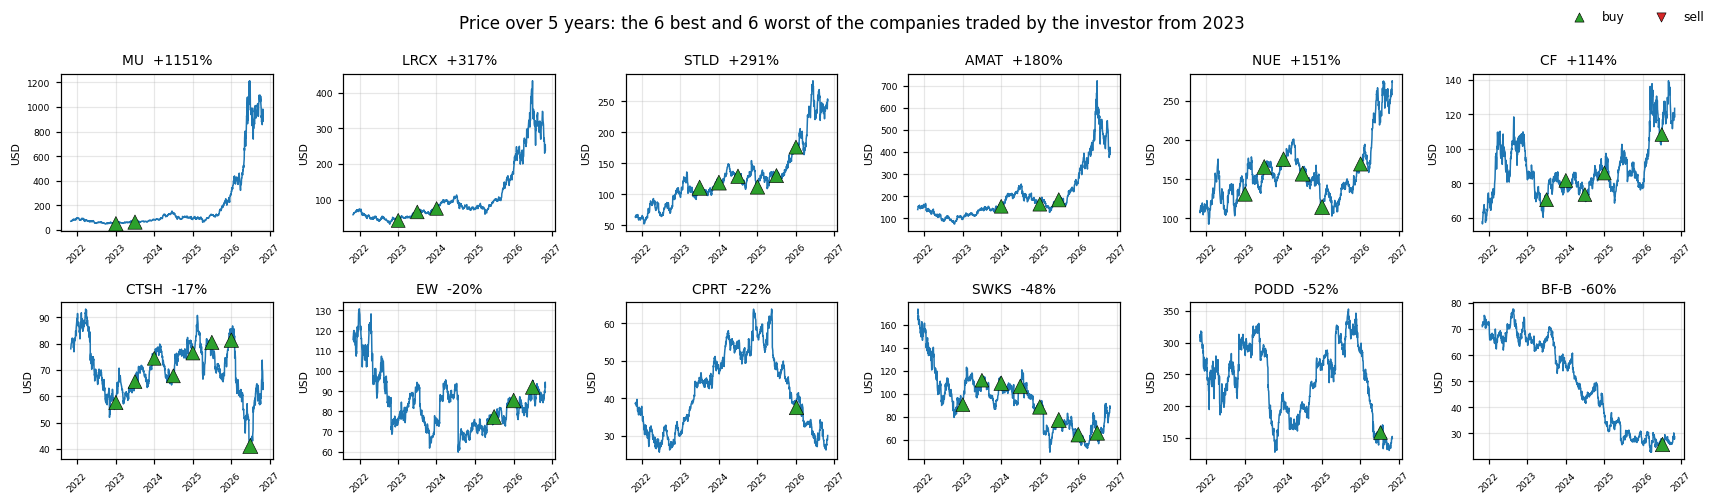
\includegraphics[width=1\textwidth]{pick_prices.png}
\caption{Share price (USD, split-adjusted, dividends excluded) over the last 5 years, one panel per company, ordered from the best to the worst price change over the period; purchases (green) and sales (red) of the investor who started in 2023, marker area in proportion to the USD traded.}
\label{fig:pick-prices}
\end{figure}
\begin{figure}[H]
\centering
\includegraphics[width=1\textwidth]{trade_amounts.png}
\caption{USD bought (green, positive) and sold (red, negative) by the investor who started in 2023, per company and decision date.}
\label{fig:trade-amounts}
\end{figure}
\section{The next picks}
\begin{table}[H]
\centering
\small
\caption{The next picks on the latest score date: score, score on the 0-to-1 scale, weight and USD of each 100 USD.}\label{tab:next}
\begin{tabular}{l l r r r r}
\hline
Company & Sector & Score & Score 0 to 1 & Weight & USD \\
\hline
First Solar (FSLR) & Technology & 34.6 & 0.93 & 11.7\% & 11.71 \\
Snap-on (SNA) & Industrials & 33.4 & 0.89 & 11.3\% & 11.29 \\
Cognizant (CTSH) & Technology & 31.4 & 0.84 & 10.6\% & 10.63 \\
ResMed (RMD) & Health care & 30.7 & 0.82 & 10.4\% & 10.37 \\
Edwards Lifesciences (EW) & Health care & 29.4 & 0.79 & 9.9\% & 9.94 \\
Skyworks Solutions (SWKS) & Technology & 29.1 & 0.78 & 9.8\% & 9.82 \\
Brown–Forman (BF-B) & Staples & 27.8 & 0.74 & 9.4\% & 9.39 \\
ON Semiconductor (ON) & Technology & 27.3 & 0.73 & 9.2\% & 9.23 \\
Insulet Corporation (PODD) & Health care & 27.0 & 0.72 & 9.1\% & 9.12 \\
Fastenal (FAST) & Industrials & 25.1 & 0.67 & 8.5\% & 8.50 \\
\hline
\end{tabular}
\end{table}
On the latest score date, 18 September 2026, the 10 highest-scoring companies are First Solar (FSLR), Snap-on (SNA), Cognizant (CTSH), ResMed (RMD), Edwards Lifesciences (EW), Skyworks Solutions (SWKS), Brown–Forman (BF-B), ON Semiconductor (ON), Insulet Corporation (PODD) and Fastenal (FAST) (Table \ref{tab:next}). Each would receive its share of the next decision's 100 USD and of any proceeds from sales. The decision is taken on the first trading day of January with the scores known then, which include the annual reports filed until that day; these picks are a preview and may change. Figure \ref{fig:next-prices} shows each pick's share price over the last 5 years, with the earlier purchases of the investor who started in 2023 and the potential purchase at today's price.

\begin{figure}[H]
\centering
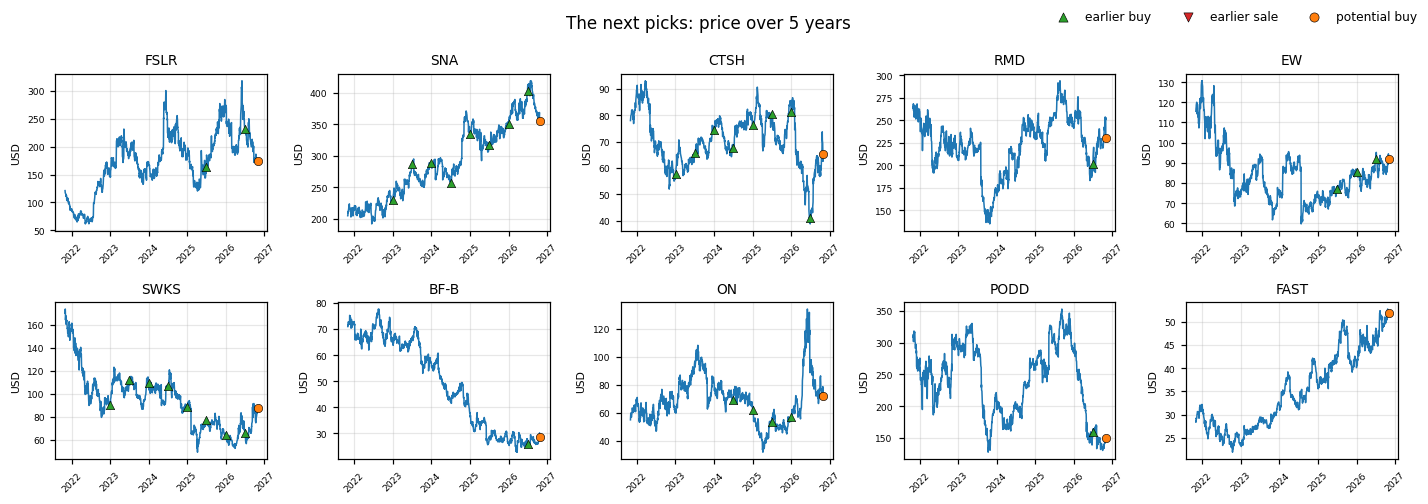
\includegraphics[width=1\textwidth]{next_prices.png}
\caption{Share price of each next pick (USD, split-adjusted, dividends excluded) over the last 5 years: earlier purchases of the investor who started in 2023 in green, the potential purchase at the latest price in orange.}
\label{fig:next-prices}
\end{figure}
\section{Winning picks we missed}
\label{sec:missed}
\begin{table}[H]
\centering
\small
\caption{Winners over the next 36 months that the score missed, by index: the share of winners held (by chance), their mean score and examples with their score on a scale from 0 to 1.}\label{tab:missed}
\begin{tabular}{l l l p{5.9cm}}
\hline
Index & Winners held (by chance) & Winners' mean score & Missed winners and their score \\
\hline
S\&P 500 & 10\% (4\%) & 0.55 & Amazon 0.08, Netflix 0.23, Constellation Brands 0.32, Adobe 0.48 \\
S\&P 400 & 5\% (9\%) & 0.42 & Paylocity 0.03, Repligen 0.16, Tenet 0.17, Qualys 0.20, Chemed 0.34 \\
S\&P 600 & 9\% (5\%) & 0.51 & Archrock 0.14, Brinker 0.16, SM Energy 0.19 \\
\hline
\end{tabular}
\end{table}
No score picks every winner, and a winner is only known afterwards. Here the winners are the ten companies with the highest return above their index over the next 36 months, found with hindsight on every date. A book of ten companies that knew nothing would hold about 4\% of them on the S\&P 500, 9\% on the S\&P 400 and 5\% on the S\&P 600 (Table \ref{tab:missed}). They are shown as a check on the rules, not as advice.

On the S\&P 500 the score holds 10\% of the winners and ranks them slightly above the median (0.55 on a scale from 0 to 1). It found the chip makers (Nvidia 0.91, Lam Research 0.96, Micron 0.91) and missed the growth platforms: Amazon 0.08, Netflix 0.23 and Constellation Brands 0.32. On the S\&P 400 the winners score below the median (0.42): Paylocity 0.03, Repligen 0.16, Tenet 0.17 and Qualys 0.20. Health care is 17\% of the winners there and 3\% of our picks. On the S\&P 600 energy companies are 24\% of the winners and 2\% of our picks.

A possible cause is in the rules. They are Graham's and Buffett's, and they reward cheap, low-debt, asset-rich companies. Many winners of the period were growth and quality companies that pay no dividend and trade at higher multiples. On the S\&P 400 they score 0.7 points lower than the average company on the dividend rule and 0.4 lower on debt cover, while our picks score 4.4 on debt cover against 2.1 for the average company. On the earlier sixteen-rule score, dropping the dividend rules made no measurable difference on the S\&P 500 and the S\&P 400, so they are not what holds the score back there; on the S\&P 600 the bands excluded zero (+0.72 and -0.93). The price rules are one more possible cause: dropping them raised the best ten on the S\&P 500, but that held on the S\&P 500 only, showed nothing on the S\&P 400 and was contradicted on the S\&P 600, so it was not adopted (Section \ref{sec:dialogue}). Companies that S\&P later added to the S\&P 500 scored lower than its existing members before they joined (0.42 against 0.51 on a scale from 0 to 1), which fits the hypothesis that the score undervalues growth; it is a hypothesis, not a tested result.

\section{Lowest scores in the index}
\label{sec:worst}
\begin{table}[H]
\centering
\small
\caption{The 10 lowest-scoring of the companies scored on the latest score date: sector, score, score on the 0-to-1 scale and colour (Green, Amber, Red or Black; not a recommendation).}\label{tab:worst}
\begin{tabular}{p{4.4cm} p{3cm} r r p{3cm}}
\hline
Company & Sector & Score & Score 0 to 1 & Colour \\
\hline
EchoStar (ECHO) & Communication Services & 0.8 & 0.03 & \cellcolor[HTML]{BFBFBF}Black \\
Palo Alto Networks (PANW) & Information Technology & 1.4 & 0.06 & \cellcolor[HTML]{BFBFBF}Black \\
GE Vernova (GEV) & Industrials & 1.6 & 0.07 & \cellcolor[HTML]{BFBFBF}Black \\
J.M. Smucker Company (The) (SJM) & Consumer Staples & 1.9 & 0.05 & \cellcolor[HTML]{BFBFBF}Black \\
Dell Technologies (DELL) & Information Technology & 2.4 & 0.07 & \cellcolor[HTML]{BFBFBF}Black \\
Exelon (EXC) & Utilities & 3.3 & 0.13 & \cellcolor[HTML]{BFBFBF}Black \\
AbbVie (ABBV) & Health Care & 3.4 & 0.09 & \cellcolor[HTML]{BFBFBF}Black \\
Cardinal Health (CAH) & Health Care & 3.6 & 0.10 & \cellcolor[HTML]{BFBFBF}Black \\
Hilton Worldwide (HLT) & Consumer Discretionary & 3.8 & 0.10 & \cellcolor[HTML]{BFBFBF}Black \\
Live Nation Entertainment (LYV) & Communication Services & 3.9 & 0.10 & \cellcolor[HTML]{BFBFBF}Black \\
\hline
\end{tabular}
\end{table}
These are the 10 lowest scores, as many as the picks, among the companies of the S\&P 500 that are scored on 18 September 2026, whether or not anyone holds them: EchoStar (ECHO), Palo Alto Networks (PANW), GE Vernova (GEV), J.M. Smucker Company (The) (SJM), Dell Technologies (DELL), Exelon (EXC), AbbVie (ABBV), Cardinal Health (CAH), Hilton Worldwide (HLT) and Live Nation Entertainment (LYV) (Table \ref{tab:worst}, prices in Figure \ref{fig:worst-prices}). Financials, Real Estate and companies with too few rules to score are not scored and so cannot appear. Companies with the same score are ordered by symbol, so when several share the last place, the alphabetically first are shown. The list shows where the score ranks these companies today; it is not a recommendation to buy, sell or sell short anything. A score of 0 means only that no rule awarded the company any points; it says nothing about what the company is worth.

The last column colours each score on the 0-to-1 scale. Green is a score above 0.6: a company one would buy. Amber is a score above 0.4 up to and including 0.6: a company one would not buy, and would hold only if already owned. Red is a score above 0.2 up to and including 0.4, and Black a score of 0.2 or less, down to 0: companies one might start to think about selling. The colours are not the rule of the wallet with sells. That rule is mechanical: at or below 0.4 it sells part of a holding, the more the lower the score, and at 0 all of it, whatever the colour. The sell signal on these companies has not been tested: no test has measured what the lowest scores did afterwards. The cut-offs are those the score uses today and are not fixed. The wallet never sells short; a short position on these companies is a later step and has not been tested.

\begin{figure}[H]
\centering
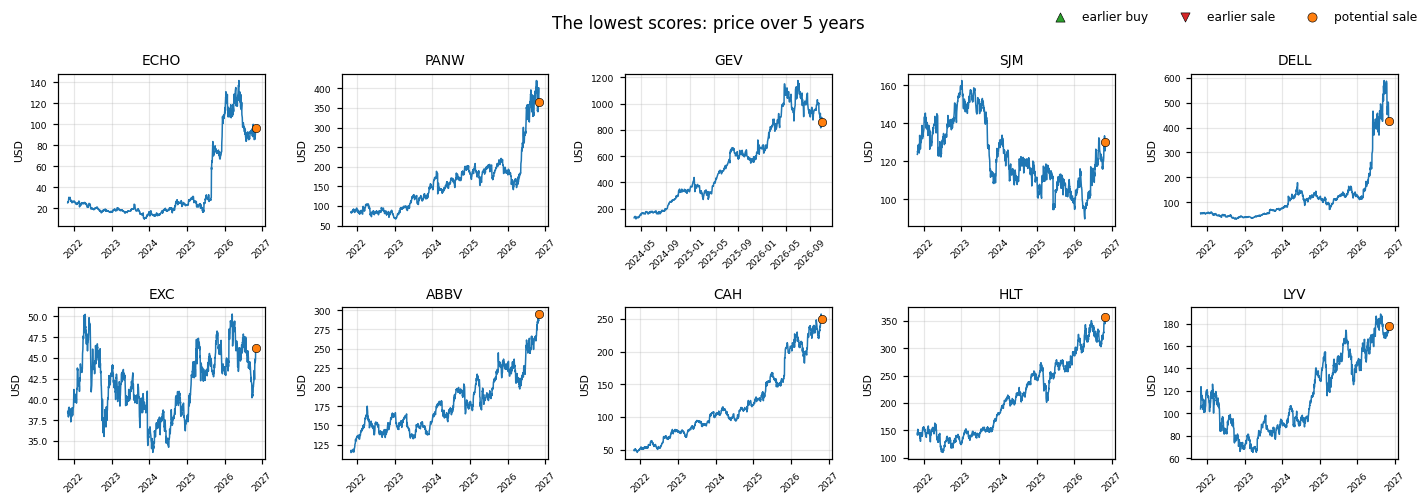
\includegraphics[width=1\textwidth]{worst_prices.png}
\caption{Share price of each of the 10 lowest scores (USD, split-adjusted, dividends excluded) over the last 5 years: earlier purchases of the investor who started in 2023 in green, earlier sales in red, the potential sale at the latest price in orange.}
\label{fig:worst-prices}
\end{figure}
\section{How the model was tested}
\label{sec:testing}
\begin{table}[H]
\centering
\small
\caption{The tests the model must pass before launch, and where each stands.}\label{tab:testing}
\begin{tabular}{l p{3.6cm} p{4.6cm} p{2.3cm}}
\hline
Test & What is checked & Result & Status \\
\hline
Winners removed & The wallet still beats its index with the 3 largest winners removed & Computed with each report: Table \ref{tab:winners} & Read from the table; in-sample \\
Company samples & Repeated samples, each leaving out a random part of the companies & S\&P 500: ahead of the index in every sample (the samples share most of their companies) & Passed on the S\&P 500, in-sample \\
Unseen companies & The score frozen, then run once on a part of the companies never used & Positive, but two companies gave 99\% of the gain (earlier sixteen-rule score) & To rerun \\
Other indices & The score beats random picks of its own index on the S\&P 400 and 600 & Not reproduced & Open \\
Two periods & The edge appears before and after 2017 & Yes on the S\&P 500 (earlier sixteen-rule score) & To rerun \\
Missed winners & Which winners the score missed, and why & Section \ref{sec:missed} & Done \\
Survivorship & The effect of companies that left the index & Not yet measured & Open \\
Real-world check & Results compared with market events and institutional logic & Not yet done & Open \\
\hline
\end{tabular}
\end{table}
This is a prototype, "first light": the first version of the model that is frozen and dated, with nothing earlier to compare it with. The figures below are in-sample stress and sampling diagnostics, compared with the index and not with random books of the same size, on a configuration that was chosen on this data after more than 100 designs were tried. The bands cover the sampling of companies only: they do not allow for the number of designs tried (multiple testing) or for the period, which the designs were chosen while looking at, so no result here is out of sample. The one held-out test, on companies the score never used, is on the earlier sixteen-rule score and is marked to rerun. The tests follow a written protocol, and a test that failed is shown as failed. The model has not cleared them: the tests below are open or failed in part. The numbers are from runs on 1 November 2026 on the ten default rules, with data as of 31 October 2026.

On the S\&P 500 the picks beat the index in every one of a set of repeated samples that each left out a random part of the companies (the samples share most of their companies, so this is not independent confirmation), by 9 to 15 points a year on average depending on the start year, and by about 5 points in the worst sample. The investor who started in 2020 earns 27.7\% a year against 15.9\% in the index. The gain is concentrated: Micron makes up 24\% and Lam Research 16\% of the 2016 investor's gain. Table \ref{tab:winners}, computed with this report, runs the wallet again with the largest winners removed as if they had never existed. The edge is present in this sample of the index but shrinks as they are removed, and it is concentrated in chip and materials companies that did well in a long bull market after 2009.

The other two indices do not confirm it as strongly: their own reports carry the same table, and it is the one to read for them. The lists of the S\&P 400 and 600 give no entry dates and lose the companies that grew into a larger index, so these two tests are biased and not yet a verdict on the rules. Companies that left the index are missing from every test, which flatters the results.

\subsection{Without the biggest winners}
\begin{table}[H]
\centering
\small
\caption{Money-weighted return a year of the wallet above the S\&P 500, in percentage points, by start year, as it is and with the largest winners removed from the ranking (computed with this report).}\label{tab:winners}
\begin{tabular}{l r r r r}
\hline
Start & As it is & Without 1 & Without 3 & Without 5 \\
\hline
2016 & +9.6 & +6.7 & +3.3 & +1.9 \\
2020 & +13.0 & +4.1 & +3.1 & +1.9 \\
2023 & +16.2 & +5.0 & +3.1 & +1.9 \\
2025 & +11.3 & +11.3 & +11.3 & +10.2 \\
\hline
\end{tabular}
\end{table}
A few companies carry much of any wallet's gain, and the next quarter may offer fewer. To see how the result would stand without them, the wallet was run again with the largest winners removed as if they had never been in the index: the companies that put the most dollars ahead of the S\&P 500 over all purchases. In order, the largest first, they are Micron Technology (MU), Lam Research (LRCX), Nvidia (NVDA), Applied Materials (AMAT) and KLA Corporation (KLAC); each column removes the first of them that its heading counts. The picks are ranked again without them, so the next-best companies fill the book on the same dates with the same money (Table \ref{tab:winners}). The scores of the remaining companies are not recomputed, and the winners were found with hindsight, so the table shows how dependent the result is on them, not what would have been picked. A column close to the first one means the gain does not rest on those companies; a column far below it means it does.

\section{Midas and the Investor}
\label{sec:dialogue}
Every result in this report was questioned before it was believed. When something looked wrong, too good, different between indices or against what a long-term investor would say, Midas, who reads the numbers, put the question to the Investor. The Investor answers only from Berkshire Hathaway's published letters to shareholders and names the year; the quotations imply no endorsement by Berkshire or Mr Buffett. Midas then tested the answer and reported back. Three of the exchanges follow. The figures in them are in-sample stress and sampling diagnostics, compared with the index and not with random books, on a configuration chosen on this data (Section \ref{sec:testing}).

\textbf{Is the dividend rule holding the score back?}

\textbf{Midas:} The winners we missed mostly pay no dividend, and they score low on the dividend rules. Should we drop them?

\textbf{The Investor:} (1984) "Berkshire has earned well over market rates on retained earnings, thereby creating over one dollar of market value for every dollar retained. Under such circumstances, any distribution would have been contrary to the financial interest of shareholders, large or small."

\textbf{Midas:} I dropped the two dividend rules from the sixteen-rule score and compared. On the S\&P 500 the best ten changed by -0.03 points a year, with a 99\% band from -1.05 to +0.41; on the S\&P 400 by -0.26. There is no measurable difference on those two indices; on the S\&P 600 the bands excluded zero (+0.72 and -0.93). The default now keeps only one dividend rule, the current dividend, and the other is a switch.

\textbf{Should a cheap price be the test of value?}

\textbf{Midas:} Dropping the P/E and price-to-book rules raised the best ten on the S\&P 500 but lowered the broad ranking, and the missed winners were growth companies. That held on the S\&P 500 only, and I did not adopt it.

\textbf{The Investor:} (1992) "Growth is always a component in the calculation of value." A low ratio of price to book value, a low price-earnings ratio or a high dividend yield are "far from determinative as to whether an investor is indeed buying something for what it is worth", and the opposite characteristics "are in no way inconsistent with a 'value' purchase". Yet "business growth, per se, tells us little about value". (2013, Graham's adage, which Buffett quotes as "Ben's adage") "Price is what you pay, value is what you get."

\textbf{Midas:} I tested a price-to-earnings-growth measure. On all three indices it widened the broad ranking a little and left the best ten slightly lower, within the noise. Used only for companies that pass the quality rule, return on equity, both rose on the S\&P 500 and the S\&P 400, by 0.3 to 1 point a year. That is small and adds complexity, so it is a switch and not the default.

\textbf{Is it too good to be true?}

\textbf{Midas:} The picks beat the index in every one of a set of repeated samples that each left out a random part of the companies. The samples share most of their companies, so that is not independent confirmation, and it still looks too good, so I removed the biggest winners as if they had never existed.

\textbf{The Investor:} (1987) "When shortages exist, however, even commodity businesses flourish", and "whenever shortages appear, the typical manager simply can't wait to expand capacity". (1989) "Time is the friend of the wonderful business, the enemy of the mediocre."

\textbf{Midas:} The 1987 passage is about insurance; I apply it to chip makers by analogy. Table \ref{tab:winners} holds the result, computed with this report: the wallet still beats the index without its largest winners, but by much less. The edge is present in this sample but thin, and it sits in chip and materials companies after 2009. Treat it with care.

\textbf{What the tests showed.} The results are for holding over years, not months: the picks are bought twice a year and not sold. The concentration is the main risk, and one or two big winners carry much of the gain, so they are treated as luck until tested the same way. The book holds ten companies, not five: ten was chosen for plausibility and diversification, although the five-company book scored higher in the tests. The tests cover the default ten rules; other switches were not tested as a set. This is what the tests showed, not advice; read the tests in Section \ref{sec:testing} before relying on a number.

\section{Where to read more}
\label{sec:reading}
\begin{table}[H]
\centering
\small
\caption{Strategy literature by risk profile.}\label{tab:reading}
\begin{tabular}{l p{4.5cm} p{5.6cm}}
\hline
Profile & Idea & Reading \\
\hline
Defensive & Preserve capital; diversified, cheap, boring; index funds & Graham, The Intelligent Investor (the defensive investor); Bogle, The Little Book of Common Sense Investing \\
Core & A wonderful company at a fair price, held for years & The Berkshire Hathaway shareholder letters; Dorsey, The Little Book That Builds Wealth \\
Value with a margin of safety & Buy at a deep discount to value & Graham (the enterprising investor); Klarman, Margin of Safety \\
Quality growth & Growth at a reasonable price, good management & Fisher, Common Stocks and Uncommon Profits; Lynch, One Up on Wall Street \\
Systematic value & Rules, ranked & Greenblatt, The Little Book That Beats the Market; Piotroski (2000), the F-score; Novy-Marx (2013), gross profitability \\
Risk awareness & Cycles and what can go wrong & Marks, The Most Important Thing; Lakonishok, Shleifer and Vishny (1994), contrarian investment \\
\hline
\end{tabular}
\end{table}
Planned, and not yet available: a member will be able to bring the strategy literature they like and ask for answers drawn from those pages, with the source named. The Berkshire Hathaway letters are free to read on the company's site. Books are copyrighted: use your own copy. The list below is grouped by the kind of risk each approach accepts. It is a starting point only: the titles are given from general knowledge and have not been checked against the books, so check each one before relying on it.

\section{Conclusions}
In this sample, the value picks bought twice a year and held are worth more today than the same money in the S\&P 500 or in Berkshire Hathaway for each of the four start years. That describes the past under rules and settings chosen while looking at it; it is not a test of the strategy. The lead is uneven: the 8 purchases of Micron Technology (MU) make up 33\% of the 2020 investor's value, and the purchases of none trail the index.

Before the strategy is used, three steps are needed: the companies that left the index must be added to the data, the score must be tested on more decisions (each quarter instead of each year), and trading costs and taxes must be included.

\newpage
\appendix
\section{Every purchase}
\label{app:purchases}
{\small
\begin{longtable}{l l l r r r r r r r}
\caption{Every purchase of the wallet with sells of the investor who started in 2020: weight in the decision's purchase, USD invested (the decision's 100 USD and the proceeds of sales), split-adjusted price at purchase and today, USD sold from it later, USD it keeps today and its total return with dividends, (sold + kept) / invested - 1.}\label{tab:purchases}\\
\hline
Year & Company & Sector & Weight & In & Bought at & Now & Sold & Kept & Return \\
\hline
\endhead
2020-01 & MU & Technology & 12\% & 12 & 55.39 & 884.74 &  & 198 & +1538\% \\
2020-01 & NUE & Materials & 12\% & 12 & 55.12 & 273.87 &  & 66 & +463\% \\
2020-01 & CTSH & Technology & 11\% & 11 & 61.92 & 65.11 &  & 13 & +17\% \\
2020-01 & SNA & Industrials & 10\% & 10 & 169.00 & 355.66 &  & 25 & +151\% \\
2020-01 & FAST & Industrials & 9\% & 9 & 18.61 & 51.91 &  & 31 & +232\% \\
2020-01 & TPR & Discretionary & 9\% & 9 & 26.93 & 116.29 & 4 & 32 & +290\% \\
2020-01 & AMAT & Technology & 9\% & 9 & 62.20 & 390.09 &  & 62 & +566\% \\
2020-01 & PKG & Materials & 9\% & 9 & 110.72 & 256.82 &  & 26 & +183\% \\
2020-01 & GILD & Health care & 9\% & 9 & 65.23 & 170.68 & 2 & 25 & +204\% \\
2020-01 & LYB & Materials & 9\% & 9 & 93.86 & 68.64 &  & 10 & +12\% \\
2020-07 & MU & Technology & 12\% & 12 & 49.70 & 884.74 &  & 217 & +1726\% \\
2020-07 & NUE & Materials & 11\% & 11 & 40.38 & 273.87 &  & 86 & +652\% \\
2020-07 & CTSH & Technology & 11\% & 11 & 56.42 & 65.11 &  & 14 & +28\% \\
2020-07 & HAS & Discretionary & 10\% & 10 & 74.69 & 119.09 & 9 & 0 & -5\% \\
2020-07 & HUM & Health care & 10\% & 10 & 391.55 & 414.50 &  & 11 & +12\% \\
2020-07 & PKG & Materials & 10\% & 10 & 99.37 & 256.82 &  & 30 & +210\% \\
2020-07 & SNA & Industrials & 9\% & 9 & 134.12 & 355.66 &  & 29 & +212\% \\
2020-07 & FAST & Industrials & 9\% & 9 & 21.50 & 51.91 &  & 26 & +184\% \\
2020-07 & TPR & Discretionary & 9\% & 9 & 12.97 & 116.29 & 9 & 64 & +699\% \\
2020-07 & HSIC & Health care & 9\% & 9 & 58.86 & 84.88 &  & 13 & +44\% \\
2021-01 & MU & Technology & 11\% & 12 & 74.05 & 884.74 &  & 142 & +1125\% \\
2021-01 & NUE & Materials & 11\% & 11 & 52.51 & 273.87 &  & 64 & +468\% \\
2021-01 & HUM & Health care & 10\% & 11 & 412.19 & 414.50 &  & 12 & +6\% \\
2021-01 & CTSH & Technology & 10\% & 10 & 79.42 & 65.11 &  & 9 & -10\% \\
2021-01 & AMAT & Technology & 10\% & 10 & 86.87 & 390.09 &  & 48 & +371\% \\
2021-01 & HAS & Discretionary & 10\% & 10 & 91.96 & 119.09 & 7 & 0 & -24\% \\
2021-01 & PKG & Materials & 10\% & 10 & 135.75 & 256.82 &  & 22 & +124\% \\
2021-01 & LRCX & Technology & 9\% & 10 & 47.80 & 239.11 &  & 52 & +430\% \\
2021-01 & GILD & Health care & 9\% & 10 & 60.11 & 170.68 & 3 & 28 & +217\% \\
2021-01 & BIIB & Health care & 9\% & 10 & 242.95 & 253.62 &  & 10 & +4\% \\
2021-07 & SNA & Industrials & 12\% & 13 & 223.42 & 355.66 &  & 23 & +83\% \\
2021-07 & MU & Technology & 11\% & 12 & 80.11 & 884.74 &  & 138 & +1033\% \\
2021-07 & HUM & Health care & 10\% & 11 & 447.63 & 414.50 &  & 11 & -2\% \\
2021-07 & CMI & Industrials & 10\% & 11 & 242.13 & 500.09 & 0 & 25 & +132\% \\
2021-07 & INTC & Technology & 10\% & 11 & 56.01 & 65.76 & 5 & 3 & -19\% \\
2021-07 & FAST & Industrials & 10\% & 11 & 26.03 & 51.91 &  & 24 & +127\% \\
2021-07 & NUE & Materials & 10\% & 11 & 96.65 & 273.87 &  & 32 & +206\% \\
2021-07 & BBY & Discretionary & 9\% & 10 & 116.37 & 95.65 & 2 & 8 & -2\% \\
2021-07 & HSIC & Health care & 9\% & 10 & 75.51 & 84.88 &  & 11 & +12\% \\
2021-07 & CTSH & Technology & 9\% & 10 & 69.84 & 65.11 &  & 10 & +2\% \\
2022-01 & SNA & Industrials & 11\% & 11 & 213.32 & 355.66 &  & 22 & +89\% \\
2022-01 & MU & Technology & 11\% & 11 & 95.75 & 884.74 &  & 102 & +845\% \\
2022-01 & HUM & Health care & 10\% & 10 & 465.45 & 414.50 &  & 10 & -6\% \\
2022-01 & CMI & Industrials & 10\% & 10 & 219.53 & 500.09 & 0 & 26 & +153\% \\
2022-01 & HSIC & Health care & 10\% & 10 & 77.43 & 84.88 &  & 11 & +10\% \\
2022-01 & INTC & Technology & 10\% & 10 & 53.21 & 65.76 & 5 & 3 & -16\% \\
2022-01 & NUE & Materials & 10\% & 10 & 113.04 & 273.87 &  & 25 & +159\% \\
2022-01 & AMAT & Technology & 10\% & 10 & 159.93 & 390.09 &  & 24 & +154\% \\
2022-01 & PKG & Materials & 9\% & 9 & 134.61 & 256.82 &  & 20 & +119\% \\
2022-01 & CTSH & Technology & 9\% & 9 & 89.57 & 65.11 &  & 7 & -21\% \\
2022-07 & SNA & Industrials & 11\% & 11 & 198.24 & 355.66 &  & 23 & +101\% \\
2022-07 & NUE & Materials & 11\% & 11 & 105.64 & 273.87 &  & 30 & +175\% \\
2022-07 & MU & Technology & 11\% & 11 & 53.65 & 884.74 &  & 179 & +1585\% \\
2022-07 & AMAT & Technology & 10\% & 10 & 86.27 & 390.09 &  & 46 & +369\% \\
2022-07 & SWKS & Technology & 10\% & 10 & 91.12 & 87.58 &  & 11 & +9\% \\
2022-07 & GOOG & Communication & 10\% & 10 & 109.08 & 278.22 &  & 25 & +157\% \\
2022-07 & GOOGL & Communication & 10\% & 10 & 108.74 & 279.84 &  & 25 & +160\% \\
2022-07 & CMI & Industrials & 10\% & 10 & 194.11 & 500.09 & 0 & 27 & +182\% \\
2022-07 & INTC & Technology & 10\% & 10 & 36.34 & 65.76 & 7 & 4 & +21\% \\
2022-07 & CTSH & Technology & 9\% & 9 & 68.03 & 65.11 &  & 10 & +3\% \\
2023-01 & MU & Technology & 11\% & 11 & 50.37 & 884.74 &  & 196 & +1683\% \\
2023-01 & SNA & Industrials & 10\% & 11 & 229.38 & 355.66 &  & 19 & +71\% \\
2023-01 & GOOG & Communication & 10\% & 11 & 89.70 & 278.22 &  & 34 & +213\% \\
2023-01 & GOOGL & Communication & 10\% & 11 & 89.12 & 279.84 &  & 34 & +217\% \\
2023-01 & NUE & Materials & 10\% & 11 & 131.06 & 273.87 &  & 24 & +120\% \\
2023-01 & CTSH & Technology & 10\% & 11 & 57.59 & 65.11 &  & 13 & +21\% \\
2023-01 & LRCX & Technology & 10\% & 10 & 41.43 & 239.11 &  & 60 & +497\% \\
2023-01 & SWKS & Technology & 10\% & 10 & 90.50 & 87.58 &  & 11 & +9\% \\
2023-01 & CMI & Industrials & 9\% & 10 & 241.04 & 500.09 & 0 & 22 & +124\% \\
2023-01 & INTC & Technology & 9\% & 10 & 26.73 & 65.76 & 10 & 6 & +61\% \\
2023-07 & STLD & Materials & 12\% & 12 & 110.78 & 250.80 &  & 29 & +137\% \\
2023-07 & NUE & Materials & 11\% & 12 & 165.61 & 273.87 &  & 20 & +73\% \\
2023-07 & SNA & Industrials & 11\% & 11 & 286.86 & 355.66 &  & 15 & +35\% \\
2023-07 & MU & Technology & 10\% & 11 & 63.90 & 884.74 &  & 149 & +1303\% \\
2023-07 & CF & Materials & 10\% & 10 & 70.43 & 123.30 &  & 19 & +88\% \\
2023-07 & DD & Industrials & 10\% & 10 & 89.84 & 140.05 &  & 17 & +66\% \\
2023-07 & CTSH & Technology & 10\% & 10 & 65.56 & 65.11 &  & 10 & +5\% \\
2023-07 & LRCX & Technology & 9\% & 10 & 65.10 & 239.11 &  & 36 & +278\% \\
2023-07 & SWKS & Technology & 9\% & 10 & 111.70 & 87.58 &  & 8 & -13\% \\
2023-07 & GOOG & Communication & 9\% & 9 & 120.56 & 278.22 &  & 22 & +133\% \\
2024-01 & STLD & Materials & 11\% & 11 & 118.91 & 250.80 &  & 25 & +119\% \\
2024-01 & NUE & Materials & 11\% & 11 & 175.43 & 273.87 &  & 18 & +62\% \\
2024-01 & SWKS & Technology & 11\% & 11 & 109.11 & 87.58 &  & 10 & -12\% \\
2024-01 & SNA & Industrials & 11\% & 11 & 288.74 & 355.66 &  & 14 & +32\% \\
2024-01 & CF & Materials & 10\% & 10 & 81.61 & 123.30 &  & 15 & +61\% \\
2024-01 & DD & Industrials & 10\% & 10 & 97.29 & 140.05 &  & 15 & +52\% \\
2024-01 & CTSH & Technology & 9\% & 10 & 74.40 & 65.11 &  & 9 & -8\% \\
2024-01 & AMAT & Technology & 9\% & 9 & 154.37 & 390.09 &  & 24 & +158\% \\
2024-01 & KEYS & Technology & 9\% & 9 & 155.49 & 307.20 &  & 19 & +98\% \\
2024-01 & LRCX & Technology & 9\% & 9 & 74.93 & 239.11 &  & 30 & +226\% \\
2024-07 & NUE & Materials & 11\% & 12 & 157.00 & 273.87 &  & 22 & +80\% \\
2024-07 & SNA & Industrials & 11\% & 11 & 256.90 & 355.66 &  & 17 & +47\% \\
2024-07 & STLD & Materials & 10\% & 11 & 129.15 & 250.80 &  & 23 & +100\% \\
2024-07 & BG & Staples & 10\% & 11 & 107.32 & 96.64 &  & 11 & -4\% \\
2024-07 & SWKS & Technology & 10\% & 11 & 106.40 & 87.58 &  & 10 & -11\% \\
2024-07 & EOG & Energy & 10\% & 11 & 126.54 & 165.54 &  & 15 & +42\% \\
2024-07 & CTSH & Technology & 10\% & 11 & 67.74 & 65.11 &  & 11 & +0\% \\
2024-07 & CF & Materials & 9\% & 10 & 73.38 & 123.30 &  & 18 & +77\% \\
2024-07 & ON & Technology & 9\% & 10 & 69.18 & 71.67 &  & 10 & +4\% \\
2024-07 & EBAY & Discretionary & 9\% & 10 & 52.68 & 121.64 & 9 & 10 & +101\% \\
2025-01 & NUE & Materials & 11\% & 12 & 114.48 & 273.87 &  & 29 & +145\% \\
2025-01 & SWKS & Technology & 10\% & 11 & 88.45 & 87.58 &  & 11 & +5\% \\
2025-01 & STLD & Materials & 10\% & 11 & 111.93 & 250.80 &  & 25 & +129\% \\
2025-01 & BG & Staples & 10\% & 11 & 77.57 & 96.64 &  & 14 & +31\% \\
2025-01 & SNA & Industrials & 10\% & 10 & 335.11 & 355.66 &  & 11 & +11\% \\
2025-01 & EOG & Energy & 10\% & 10 & 124.71 & 165.54 &  & 15 & +42\% \\
2025-01 & CTSH & Technology & 10\% & 10 & 76.41 & 65.11 &  & 9 & -12\% \\
2025-01 & AMAT & Technology & 9\% & 10 & 163.87 & 390.09 &  & 24 & +141\% \\
2025-01 & ON & Technology & 9\% & 10 & 61.71 & 71.67 &  & 11 & +16\% \\
2025-01 & CF & Materials & 9\% & 10 & 85.83 & 123.30 &  & 14 & +49\% \\
2025-07 & ON & Technology & 11\% & 13 & 53.60 & 71.67 &  & 17 & +34\% \\
2025-07 & SWKS & Technology & 11\% & 13 & 77.16 & 87.58 &  & 15 & +18\% \\
2025-07 & SNA & Industrials & 11\% & 13 & 317.86 & 355.66 &  & 15 & +16\% \\
2025-07 & EW & Health care & 10\% & 12 & 77.18 & 92.01 &  & 14 & +19\% \\
2025-07 & BG & Staples & 10\% & 11 & 80.25 & 96.64 &  & 14 & +25\% \\
2025-07 & FSLR & Technology & 10\% & 11 & 162.96 & 174.40 &  & 12 & +7\% \\
2025-07 & CTSH & Technology & 10\% & 11 & 80.44 & 65.11 &  & 9 & -17\% \\
2025-07 & AMAT & Technology & 9\% & 11 & 183.76 & 390.09 &  & 23 & +114\% \\
2025-07 & STLD & Materials & 9\% & 11 & 130.16 & 250.80 &  & 21 & +95\% \\
2025-07 & EOG & Energy & 9\% & 11 & 121.19 & 165.54 &  & 15 & +43\% \\
2026-01 & ON & Technology & 11\% & 13 & 56.70 & 71.67 &  & 16 & +26\% \\
2026-01 & SNA & Industrials & 11\% & 12 & 350.95 & 355.66 &  & 13 & +3\% \\
2026-01 & SWKS & Technology & 10\% & 12 & 64.40 & 87.58 &  & 16 & +39\% \\
2026-01 & EW & Health care & 10\% & 12 & 85.33 & 92.01 &  & 13 & +8\% \\
2026-01 & CPRT & Industrials & 10\% & 11 & 37.77 & 30.13 &  & 9 & -20\% \\
2026-01 & CTSH & Technology & 10\% & 11 & 81.28 & 65.11 &  & 9 & -18\% \\
2026-01 & BG & Staples & 10\% & 11 & 92.64 & 96.64 &  & 12 & +6\% \\
2026-01 & EOG & Energy & 10\% & 11 & 107.27 & 165.54 &  & 17 & +59\% \\
2026-01 & NUE & Materials & 10\% & 11 & 169.40 & 273.87 &  & 18 & +63\% \\
2026-01 & STLD & Materials & 9\% & 10 & 176.06 & 250.80 &  & 15 & +44\% \\
2026-07 & SNA & Industrials & 11\% & 12 & 403.28 & 355.66 &  & 11 & -11\% \\
2026-07 & CTSH & Technology & 11\% & 12 & 41.07 & 65.11 &  & 19 & +59\% \\
2026-07 & FSLR & Technology & 11\% & 11 & 232.08 & 174.40 &  & 9 & -25\% \\
2026-07 & SWKS & Technology & 10\% & 11 & 65.93 & 87.58 &  & 15 & +33\% \\
2026-07 & RMD & Health care & 10\% & 11 & 201.10 & 229.94 &  & 13 & +15\% \\
2026-07 & EW & Health care & 10\% & 11 & 91.99 & 92.01 &  & 11 & +0\% \\
2026-07 & BF-B & Staples & 10\% & 11 & 25.83 & 28.71 &  & 12 & +12\% \\
2026-07 & PODD & Health care & 9\% & 10 & 159.79 & 149.68 &  & 9 & -6\% \\
2026-07 & CF & Materials & 9\% & 10 & 108.16 & 123.30 &  & 11 & +15\% \\
2026-07 & HUM & Health care & 9\% & 9 & 409.42 & 414.50 &  & 9 & +1\% \\
\hline
\end{longtable}}
\section{Every company ranked}
\label{app:ranking}
{\small
\begin{longtable}{r p{4.4cm} p{2.8cm} r r l l}
\caption{All 379 companies of the S\&P 500 scored on 18 September 2026, from the highest score on the 0-to-1 scale to the lowest: sector, that score, the score, colour (Green, Amber, Red or Black; not a recommendation) and whether the company is one of the next picks.}\label{tab:ranking}\\
\hline
Rank & Company & Sector & Score 0 to 1 & Score & Colour & Next pick \\
\hline
\endhead
1 & Supermicro (SMCI) & Information Technology & 0.96 & 23.9 & \cellcolor[HTML]{C6EFCE}Green &  \\
2 & First Solar (FSLR) & Information Technology & 0.93 & 34.6 & \cellcolor[HTML]{C6EFCE}Green & Pick \\
3 & Deckers Brands (DECK) & Consumer Discretionary & 0.92 & 23.0 & \cellcolor[HTML]{C6EFCE}Green &  \\
4 & Snap-on (SNA) & Industrials & 0.89 & 33.4 & \cellcolor[HTML]{C6EFCE}Green & Pick \\
5 & PulteGroup (PHM) & Consumer Discretionary & 0.88 & 15.2 & \cellcolor[HTML]{C6EFCE}Green &  \\
6 & Lululemon Athletica (LULU) & Consumer Discretionary & 0.86 & 21.5 & \cellcolor[HTML]{C6EFCE}Green &  \\
7 & A. O. Smith (AOS) & Industrials & 0.84 & 23.3 & \cellcolor[HTML]{C6EFCE}Green &  \\
8 & Cognizant (CTSH) & Information Technology & 0.84 & 31.4 & \cellcolor[HTML]{C6EFCE}Green & Pick \\
9 & Nike, Inc. (NKE) & Consumer Discretionary & 0.84 & 23.3 & \cellcolor[HTML]{C6EFCE}Green &  \\
10 & Copart (CPRT) & Industrials & 0.84 & 21.0 & \cellcolor[HTML]{C6EFCE}Green &  \\
11 & ResMed (RMD) & Health Care & 0.82 & 30.7 & \cellcolor[HTML]{C6EFCE}Green & Pick \\
12 & Ralph Lauren Corporation (RL) & Consumer Discretionary & 0.80 & 22.2 & \cellcolor[HTML]{C6EFCE}Green &  \\
13 & Regeneron Pharmaceuticals (REGN) & Health Care & 0.79 & 22.1 & \cellcolor[HTML]{C6EFCE}Green &  \\
14 & Accenture (ACN) & Information Technology & 0.79 & 22.0 & \cellcolor[HTML]{C6EFCE}Green &  \\
15 & Fox Corporation (Class B) (FOX) & Communication Services & 0.79 & 21.8 & \cellcolor[HTML]{C6EFCE}Green &  \\
16 & Fox Corporation (Class A) (FOXA) & Communication Services & 0.79 & 21.8 & \cellcolor[HTML]{C6EFCE}Green &  \\
17 & Edwards Lifesciences (EW) & Health Care & 0.79 & 29.4 & \cellcolor[HTML]{C6EFCE}Green & Pick \\
18 & Skyworks Solutions (SWKS) & Information Technology & 0.78 & 29.1 & \cellcolor[HTML]{C6EFCE}Green & Pick \\
19 & Airbnb (ABNB) & Consumer Discretionary & 0.77 & 15.7 & \cellcolor[HTML]{C6EFCE}Green &  \\
20 & Meta Platforms (META) & Communication Services & 0.76 & 21.1 & \cellcolor[HTML]{C6EFCE}Green &  \\
21 & Brown–Forman (BF-B) & Consumer Staples & 0.74 & 27.8 & \cellcolor[HTML]{C6EFCE}Green & Pick \\
22 & ON Semiconductor (ON) & Information Technology & 0.73 & 27.3 & \cellcolor[HTML]{C6EFCE}Green & Pick \\
23 & Insulet Corporation (PODD) & Health Care & 0.72 & 27.0 & \cellcolor[HTML]{C6EFCE}Green & Pick \\
24 & Incyte (INCY) & Health Care & 0.70 & 17.5 & \cellcolor[HTML]{C6EFCE}Green &  \\
25 & Garmin (GRMN) & Consumer Discretionary & 0.68 & 17.1 & \cellcolor[HTML]{C6EFCE}Green &  \\
26 & Freeport-McMoRan (FCX) & Materials & 0.68 & 17.3 & \cellcolor[HTML]{C6EFCE}Green &  \\
27 & Fastenal (FAST) & Industrials & 0.67 & 25.1 & \cellcolor[HTML]{C6EFCE}Green & Pick \\
28 & Zoetis (ZTS) & Health Care & 0.67 & 25.1 & \cellcolor[HTML]{C6EFCE}Green &  \\
29 & News Corp (Class A) (NWSA) & Communication Services & 0.66 & 18.4 & \cellcolor[HTML]{C6EFCE}Green &  \\
30 & Hormel Foods (HRL) & Consumer Staples & 0.66 & 18.3 & \cellcolor[HTML]{C6EFCE}Green &  \\
31 & CF Industries (CF) & Materials & 0.66 & 24.7 & \cellcolor[HTML]{C6EFCE}Green &  \\
32 & EOG Resources (EOG) & Energy & 0.65 & 24.5 & \cellcolor[HTML]{C6EFCE}Green &  \\
33 & Aptiv (APTV) & Consumer Discretionary & 0.65 & 24.4 & \cellcolor[HTML]{C6EFCE}Green &  \\
34 & Bunge Global (BG) & Consumer Staples & 0.65 & 22.5 & \cellcolor[HTML]{C6EFCE}Green &  \\
35 & West Pharmaceutical Services (WST) & Health Care & 0.65 & 24.1 & \cellcolor[HTML]{C6EFCE}Green &  \\
36 & W. W. Grainger (GWW) & Industrials & 0.64 & 23.9 & \cellcolor[HTML]{C6EFCE}Green &  \\
37 & Dover Corporation (DOV) & Industrials & 0.64 & 23.9 & \cellcolor[HTML]{C6EFCE}Green &  \\
38 & News Corp (Class B) (NWS) & Communication Services & 0.63 & 17.5 & \cellcolor[HTML]{C6EFCE}Green &  \\
39 & Humana (HUM) & Health Care & 0.63 & 23.5 & \cellcolor[HTML]{C6EFCE}Green &  \\
40 & Steel Dynamics (STLD) & Materials & 0.63 & 23.4 & \cellcolor[HTML]{C6EFCE}Green &  \\
41 & Applied Materials (AMAT) & Information Technology & 0.62 & 23.3 & \cellcolor[HTML]{C6EFCE}Green &  \\
42 & PPG Industries (PPG) & Materials & 0.62 & 23.2 & \cellcolor[HTML]{C6EFCE}Green &  \\
43 & Nucor (NUE) & Materials & 0.61 & 23.0 & \cellcolor[HTML]{C6EFCE}Green &  \\
44 & CRH plc (CRH) & Materials & 0.61 & 21.1 & \cellcolor[HTML]{C6EFCE}Green &  \\
45 & Carvana (CVNA) & Consumer Discretionary & 0.61 & 16.9 & \cellcolor[HTML]{C6EFCE}Green &  \\
46 & Qualcomm (QCOM) & Information Technology & 0.61 & 22.7 & \cellcolor[HTML]{C6EFCE}Green &  \\
47 & Veeva Systems (VEEV) & Health Care & 0.60 & 15.1 & \cellcolor[HTML]{C6EFCE}Green &  \\
48 & Ferguson Enterprises (FERG) & Industrials & 0.60 & 20.9 & \cellcolor[HTML]{C6EFCE}Green &  \\
49 & Nvidia (NVDA) & Information Technology & 0.60 & 22.5 & \cellcolor[HTML]{C6EFCE}Green &  \\
50 & Halliburton (HAL) & Energy & 0.60 & 15.3 & \cellcolor[HTML]{C6EFCE}Green &  \\
51 & Intuit (INTU) & Information Technology & 0.60 & 22.5 & \cellcolor[HTML]{C6EFCE}Green &  \\
52 & Abbott Laboratories (ABT) & Health Care & 0.60 & 22.3 & \cellcolor[HTML]{FFEB9C}Amber &  \\
53 & Pentair (PNR) & Industrials & 0.60 & 22.3 & \cellcolor[HTML]{FFEB9C}Amber &  \\
54 & Tractor Supply (TSCO) & Consumer Discretionary & 0.59 & 22.0 & \cellcolor[HTML]{FFEB9C}Amber &  \\
55 & Martin Marietta Materials (MLM) & Materials & 0.59 & 21.9 & \cellcolor[HTML]{FFEB9C}Amber &  \\
56 & Biogen (BIIB) & Health Care & 0.58 & 21.7 & \cellcolor[HTML]{FFEB9C}Amber &  \\
57 & Elevance Health (ELV) & Health Care & 0.58 & 21.7 & \cellcolor[HTML]{FFEB9C}Amber &  \\
58 & Lam Research (LRCX) & Information Technology & 0.57 & 21.4 & \cellcolor[HTML]{FFEB9C}Amber &  \\
59 & Alphabet Inc. (Class C) (GOOG) & Communication Services & 0.57 & 21.4 & \cellcolor[HTML]{FFEB9C}Amber &  \\
60 & Alphabet Inc. (Class A) (GOOGL) & Communication Services & 0.57 & 21.4 & \cellcolor[HTML]{FFEB9C}Amber &  \\
61 & Xylem Inc. (XYL) & Industrials & 0.57 & 21.4 & \cellcolor[HTML]{FFEB9C}Amber &  \\
62 & General Dynamics (GD) & Industrials & 0.57 & 21.4 & \cellcolor[HTML]{FFEB9C}Amber &  \\
63 & Archer Daniels Midland (ADM) & Consumer Staples & 0.57 & 21.3 & \cellcolor[HTML]{FFEB9C}Amber &  \\
64 & Zimmer Biomet (ZBH) & Health Care & 0.57 & 21.2 & \cellcolor[HTML]{FFEB9C}Amber &  \\
65 & Intuitive Surgical (ISRG) & Health Care & 0.56 & 14.1 & \cellcolor[HTML]{FFEB9C}Amber &  \\
66 & Leidos (LDOS) & Industrials & 0.56 & 21.0 & \cellcolor[HTML]{FFEB9C}Amber &  \\
67 & Old Dominion (ODFL) & Industrials & 0.56 & 21.0 & \cellcolor[HTML]{FFEB9C}Amber &  \\
68 & Lennox International (LII) & Industrials & 0.56 & 20.8 & \cellcolor[HTML]{FFEB9C}Amber &  \\
69 & GE HealthCare (GEHC) & Health Care & 0.56 & 19.2 & \cellcolor[HTML]{FFEB9C}Amber &  \\
70 & NXP Semiconductors (NXPI) & Information Technology & 0.55 & 20.6 & \cellcolor[HTML]{FFEB9C}Amber &  \\
71 & Valero Energy (VLO) & Energy & 0.55 & 20.5 & \cellcolor[HTML]{FFEB9C}Amber &  \\
72 & KLA Corporation (KLAC) & Information Technology & 0.55 & 20.4 & \cellcolor[HTML]{FFEB9C}Amber &  \\
73 & Hubbell Incorporated (HUBB) & Industrials & 0.55 & 20.4 & \cellcolor[HTML]{FFEB9C}Amber &  \\
74 & Sandisk (SNDK) & Information Technology & 0.54 & 18.8 & \cellcolor[HTML]{FFEB9C}Amber &  \\
75 & Align Technology (ALGN) & Health Care & 0.54 & 13.6 & \cellcolor[HTML]{FFEB9C}Amber &  \\
76 & Ross Stores (ROST) & Consumer Discretionary & 0.54 & 20.2 & \cellcolor[HTML]{FFEB9C}Amber &  \\
77 & Veralto (VLTO) & Industrials & 0.54 & 18.6 & \cellcolor[HTML]{FFEB9C}Amber &  \\
78 & Cummins (CMI) & Industrials & 0.54 & 20.1 & \cellcolor[HTML]{FFEB9C}Amber &  \\
79 & Moderna (MRNA) & Health Care & 0.54 & 20.0 & \cellcolor[HTML]{FFEB9C}Amber &  \\
80 & IDEX Corporation (IEX) & Industrials & 0.53 & 19.9 & \cellcolor[HTML]{FFEB9C}Amber &  \\
81 & Expeditors International (EXPD) & Industrials & 0.53 & 13.3 & \cellcolor[HTML]{FFEB9C}Amber &  \\
82 & Chipotle Mexican Grill (CMG) & Consumer Discretionary & 0.53 & 19.9 & \cellcolor[HTML]{FFEB9C}Amber &  \\
83 & Schlumberger (SLB) & Energy & 0.53 & 19.8 & \cellcolor[HTML]{FFEB9C}Amber &  \\
84 & Allegion (ALLE) & Industrials & 0.53 & 19.8 & \cellcolor[HTML]{FFEB9C}Amber &  \\
85 & TE Connectivity (TEL) & Information Technology & 0.53 & 19.8 & \cellcolor[HTML]{FFEB9C}Amber &  \\
86 & CrowdStrike (CRWD) & Information Technology & 0.53 & 14.6 & \cellcolor[HTML]{FFEB9C}Amber &  \\
87 & Newmont (NEM) & Materials & 0.52 & 19.4 & \cellcolor[HTML]{FFEB9C}Amber &  \\
88 & Packaging Corporation of America (PKG) & Materials & 0.52 & 19.4 & \cellcolor[HTML]{FFEB9C}Amber &  \\
89 & General Motors (GM) & Consumer Discretionary & 0.52 & 12.9 & \cellcolor[HTML]{FFEB9C}Amber &  \\
90 & Amphenol (APH) & Information Technology & 0.52 & 19.3 & \cellcolor[HTML]{FFEB9C}Amber &  \\
91 & Baker Hughes (BKR) & Energy & 0.51 & 13.1 & \cellcolor[HTML]{FFEB9C}Amber &  \\
92 & Bio-Techne (TECH) & Health Care & 0.51 & 19.2 & \cellcolor[HTML]{FFEB9C}Amber &  \\
93 & Steris (STE) & Health Care & 0.51 & 19.2 & \cellcolor[HTML]{FFEB9C}Amber &  \\
94 & Stryker Corporation (SYK) & Health Care & 0.51 & 19.1 & \cellcolor[HTML]{FFEB9C}Amber &  \\
95 & Medtronic (MDT) & Health Care & 0.51 & 19.1 & \cellcolor[HTML]{FFEB9C}Amber &  \\
96 & Arista Networks (ANET) & Information Technology & 0.51 & 12.8 & \cellcolor[HTML]{FFEB9C}Amber &  \\
97 & Agilent Technologies (A) & Health Care & 0.51 & 19.1 & \cellcolor[HTML]{FFEB9C}Amber &  \\
98 & Microsoft (MSFT) & Information Technology & 0.51 & 19.0 & \cellcolor[HTML]{FFEB9C}Amber &  \\
99 & TJX Companies (TJX) & Consumer Discretionary & 0.50 & 18.9 & \cellcolor[HTML]{FFEB9C}Amber &  \\
100 & Western Digital (WDC) & Information Technology & 0.50 & 18.8 & \cellcolor[HTML]{FFEB9C}Amber &  \\
101 & Ball Corporation (BALL) & Materials & 0.50 & 18.7 & \cellcolor[HTML]{FFEB9C}Amber &  \\
102 & Advanced Micro Devices (AMD) & Information Technology & 0.50 & 18.6 & \cellcolor[HTML]{FFEB9C}Amber &  \\
103 & Mosaic Company (The) (MOS) & Materials & 0.50 & 18.6 & \cellcolor[HTML]{FFEB9C}Amber &  \\
104 & Best Buy (BBY) & Consumer Discretionary & 0.50 & 18.6 & \cellcolor[HTML]{FFEB9C}Amber &  \\
105 & Texas Instruments (TXN) & Information Technology & 0.49 & 18.5 & \cellcolor[HTML]{FFEB9C}Amber &  \\
106 & Vulcan Materials Company (VMC) & Materials & 0.49 & 18.4 & \cellcolor[HTML]{FFEB9C}Amber &  \\
107 & Monolithic Power Systems (MPWR) & Information Technology & 0.49 & 12.2 & \cellcolor[HTML]{FFEB9C}Amber &  \\
108 & FedEx (FDX) & Industrials & 0.49 & 18.2 & \cellcolor[HTML]{FFEB9C}Amber &  \\
109 & Sempra (SRE) & Utilities & 0.49 & 18.2 & \cellcolor[HTML]{FFEB9C}Amber &  \\
110 & Flex Ltd. (FLEX) & Information Technology & 0.49 & 18.2 & \cellcolor[HTML]{FFEB9C}Amber &  \\
111 & Tesla, Inc. (TSLA) & Consumer Discretionary & 0.48 & 18.1 & \cellcolor[HTML]{FFEB9C}Amber &  \\
112 & Smurfit Westrock (SW) & Materials & 0.48 & 16.8 & \cellcolor[HTML]{FFEB9C}Amber &  \\
113 & Akamai Technologies (AKAM) & Information Technology & 0.48 & 12.1 & \cellcolor[HTML]{FFEB9C}Amber &  \\
114 & LyondellBasell (LYB) & Materials & 0.48 & 18.1 & \cellcolor[HTML]{FFEB9C}Amber &  \\
115 & Ingersoll Rand (IR) & Industrials & 0.48 & 18.0 & \cellcolor[HTML]{FFEB9C}Amber &  \\
116 & Cintas (CTAS) & Industrials & 0.48 & 18.0 & \cellcolor[HTML]{FFEB9C}Amber &  \\
117 & United Parcel Service (UPS) & Industrials & 0.48 & 13.4 & \cellcolor[HTML]{FFEB9C}Amber &  \\
118 & Axon Enterprise (AXON) & Industrials & 0.48 & 18.0 & \cellcolor[HTML]{FFEB9C}Amber &  \\
119 & Waters Corporation (WAT) & Health Care & 0.48 & 17.9 & \cellcolor[HTML]{FFEB9C}Amber &  \\
120 & Ulta Beauty (ULTA) & Consumer Discretionary & 0.47 & 11.9 & \cellcolor[HTML]{FFEB9C}Amber &  \\
121 & Sysco (SYY) & Consumer Staples & 0.47 & 17.7 & \cellcolor[HTML]{FFEB9C}Amber &  \\
122 & ConocoPhillips (COP) & Energy & 0.47 & 17.7 & \cellcolor[HTML]{FFEB9C}Amber &  \\
123 & Comcast (CMCSA) & Communication Services & 0.47 & 13.1 & \cellcolor[HTML]{FFEB9C}Amber &  \\
124 & Baxter International (BAX) & Health Care & 0.47 & 17.7 & \cellcolor[HTML]{FFEB9C}Amber &  \\
125 & Teledyne Technologies (TDY) & Information Technology & 0.47 & 17.6 & \cellcolor[HTML]{FFEB9C}Amber &  \\
126 & CDW Corporation (CDW) & Information Technology & 0.47 & 17.6 & \cellcolor[HTML]{FFEB9C}Amber &  \\
127 & APA Corporation (APA) & Energy & 0.47 & 17.6 & \cellcolor[HTML]{FFEB9C}Amber &  \\
128 & Devon Energy (DVN) & Energy & 0.47 & 17.6 & \cellcolor[HTML]{FFEB9C}Amber &  \\
129 & Caterpillar Inc. (CAT) & Industrials & 0.47 & 17.5 & \cellcolor[HTML]{FFEB9C}Amber &  \\
130 & Tapestry, Inc. (TPR) & Consumer Discretionary & 0.47 & 17.4 & \cellcolor[HTML]{FFEB9C}Amber &  \\
131 & Solventum (SOLV) & Health Care & 0.46 & 16.1 & \cellcolor[HTML]{FFEB9C}Amber &  \\
132 & Comfort Systems USA (FIX) & Industrials & 0.46 & 17.4 & \cellcolor[HTML]{FFEB9C}Amber &  \\
133 & Automatic Data Processing (ADP) & Industrials & 0.46 & 17.2 & \cellcolor[HTML]{FFEB9C}Amber &  \\
134 & Coherent Corp. (COHR) & Information Technology & 0.46 & 17.2 & \cellcolor[HTML]{FFEB9C}Amber &  \\
135 & Vertex Pharmaceuticals (VRTX) & Health Care & 0.46 & 11.5 & \cellcolor[HTML]{FFEB9C}Amber &  \\
136 & Boston Scientific (BSX) & Health Care & 0.46 & 17.1 & \cellcolor[HTML]{FFEB9C}Amber &  \\
137 & Ciena (CIEN) & Information Technology & 0.45 & 17.0 & \cellcolor[HTML]{FFEB9C}Amber &  \\
138 & Datadog (DDOG) & Information Technology & 0.45 & 7.0 & \cellcolor[HTML]{FFEB9C}Amber &  \\
139 & AppLovin (APP) & Communication Services & 0.45 & 16.9 & \cellcolor[HTML]{FFEB9C}Amber &  \\
140 & Phillips 66 (PSX) & Energy & 0.45 & 16.7 & \cellcolor[HTML]{FFEB9C}Amber &  \\
141 & Keysight Technologies (KEYS) & Information Technology & 0.45 & 16.7 & \cellcolor[HTML]{FFEB9C}Amber &  \\
142 & Lumentum (LITE) & Information Technology & 0.44 & 16.6 & \cellcolor[HTML]{FFEB9C}Amber &  \\
143 & C.H. Robinson (CHRW) & Industrials & 0.44 & 16.6 & \cellcolor[HTML]{FFEB9C}Amber &  \\
144 & Nordson Corporation (NDSN) & Industrials & 0.44 & 16.5 & \cellcolor[HTML]{FFEB9C}Amber &  \\
145 & MGM Resorts (MGM) & Consumer Discretionary & 0.44 & 16.5 & \cellcolor[HTML]{FFEB9C}Amber &  \\
146 & Marathon Petroleum (MPC) & Energy & 0.44 & 16.4 & \cellcolor[HTML]{FFEB9C}Amber &  \\
147 & Fortinet (FTNT) & Information Technology & 0.44 & 16.3 & \cellcolor[HTML]{FFEB9C}Amber &  \\
148 & Paychex (PAYX) & Industrials & 0.43 & 16.2 & \cellcolor[HTML]{FFEB9C}Amber &  \\
149 & Cooper Companies (The) (COO) & Health Care & 0.43 & 16.1 & \cellcolor[HTML]{FFEB9C}Amber &  \\
150 & Public Service Enterprise Group (PEG) & Utilities & 0.43 & 16.1 & \cellcolor[HTML]{FFEB9C}Amber &  \\
151 & AT\&T (T) & Communication Services & 0.43 & 16.1 & \cellcolor[HTML]{FFEB9C}Amber &  \\
152 & Henry Schein (HSIC) & Health Care & 0.43 & 16.0 & \cellcolor[HTML]{FFEB9C}Amber &  \\
153 & Jacobs Solutions (J) & Industrials & 0.42 & 15.8 & \cellcolor[HTML]{FFEB9C}Amber &  \\
154 & NetApp (NTAP) & Information Technology & 0.42 & 15.8 & \cellcolor[HTML]{FFEB9C}Amber &  \\
155 & Dollar General (DG) & Consumer Staples & 0.42 & 15.8 & \cellcolor[HTML]{FFEB9C}Amber &  \\
156 & Universal Health Services (UHS) & Health Care & 0.42 & 11.7 & \cellcolor[HTML]{FFEB9C}Amber &  \\
157 & Honeywell Technologies (HON) & Industrials & 0.42 & 15.7 & \cellcolor[HTML]{FFEB9C}Amber &  \\
158 & Constellation Energy (CEG) & Utilities & 0.42 & 15.7 & \cellcolor[HTML]{FFEB9C}Amber &  \\
159 & Huntington Ingalls Industries (HII) & Industrials & 0.42 & 15.6 & \cellcolor[HTML]{FFEB9C}Amber &  \\
160 & Amcor (AMCR) & Materials & 0.41 & 15.5 & \cellcolor[HTML]{FFEB9C}Amber &  \\
161 & Lilly (Eli) (LLY) & Health Care & 0.41 & 15.5 & \cellcolor[HTML]{FFEB9C}Amber &  \\
162 & Micron Technology (MU) & Information Technology & 0.41 & 15.4 & \cellcolor[HTML]{FFEB9C}Amber &  \\
163 & AES Corporation (AES) & Utilities & 0.41 & 10.3 & \cellcolor[HTML]{FFEB9C}Amber &  \\
164 & Eaton Corporation (ETN) & Industrials & 0.41 & 15.3 & \cellcolor[HTML]{FFEB9C}Amber &  \\
165 & Carrier Global (CARR) & Industrials & 0.41 & 15.3 & \cellcolor[HTML]{FFEB9C}Amber &  \\
166 & Air Products (APD) & Materials & 0.41 & 10.2 & \cellcolor[HTML]{FFEB9C}Amber &  \\
167 & Howmet Aerospace (HWM) & Industrials & 0.41 & 14.1 & \cellcolor[HTML]{FFEB9C}Amber &  \\
168 & Seagate Technology (STX) & Information Technology & 0.41 & 15.2 & \cellcolor[HTML]{FFEB9C}Amber &  \\
169 & Parker Hannifin (PH) & Industrials & 0.41 & 15.2 & \cellcolor[HTML]{FFEB9C}Amber &  \\
170 & Broadridge Financial Solutions (BR) & Industrials & 0.40 & 15.1 & \cellcolor[HTML]{FFEB9C}Amber &  \\
171 & Merck \& Co. (MRK) & Health Care & 0.40 & 15.1 & \cellcolor[HTML]{FFEB9C}Amber &  \\
172 & Masco (MAS) & Industrials & 0.40 & 15.1 & \cellcolor[HTML]{FFEB9C}Amber &  \\
173 & DuPont (DD) & Industrials & 0.40 & 15.0 & \cellcolor[HTML]{FFEB9C}Amber &  \\
174 & T-Mobile US (TMUS) & Communication Services & 0.40 & 14.9 & \cellcolor[HTML]{F4B6B6}Red &  \\
175 & Generac (GNRC) & Industrials & 0.40 & 14.8 & \cellcolor[HTML]{F4B6B6}Red &  \\
176 & Synopsys (SNPS) & Information Technology & 0.40 & 14.8 & \cellcolor[HTML]{F4B6B6}Red &  \\
177 & Edison International (EIX) & Utilities & 0.39 & 14.7 & \cellcolor[HTML]{F4B6B6}Red &  \\
178 & Omnicom Group (OMC) & Communication Services & 0.39 & 14.7 & \cellcolor[HTML]{F4B6B6}Red &  \\
179 & Qnity Electronics (Q) & Information Technology & 0.39 & 13.6 & \cellcolor[HTML]{F4B6B6}Red &  \\
180 & Genuine Parts Company (GPC) & Consumer Discretionary & 0.39 & 14.7 & \cellcolor[HTML]{F4B6B6}Red &  \\
181 & Dexcom (DXCM) & Health Care & 0.39 & 9.7 & \cellcolor[HTML]{F4B6B6}Red &  \\
182 & Workday, Inc. (WDAY) & Information Technology & 0.39 & 10.8 & \cellcolor[HTML]{F4B6B6}Red &  \\
183 & Diamondback Energy (FANG) & Energy & 0.39 & 14.5 & \cellcolor[HTML]{F4B6B6}Red &  \\
184 & Danaher Corporation (DHR) & Health Care & 0.38 & 14.4 & \cellcolor[HTML]{F4B6B6}Red &  \\
185 & Gilead Sciences (GILD) & Health Care & 0.38 & 14.4 & \cellcolor[HTML]{F4B6B6}Red &  \\
186 & Williams-Sonoma, Inc. (WSM) & Consumer Discretionary & 0.38 & 9.6 & \cellcolor[HTML]{F4B6B6}Red &  \\
187 & Vertiv (VRT) & Industrials & 0.38 & 14.3 & \cellcolor[HTML]{F4B6B6}Red &  \\
188 & Expand Energy (EXE) & Energy & 0.38 & 13.1 & \cellcolor[HTML]{F4B6B6}Red &  \\
189 & Verizon (VZ) & Communication Services & 0.38 & 14.2 & \cellcolor[HTML]{F4B6B6}Red &  \\
190 & Uber (UBER) & Industrials & 0.38 & 14.2 & \cellcolor[HTML]{F4B6B6}Red &  \\
191 & Booking Holdings (BKNG) & Consumer Discretionary & 0.38 & 12.5 & \cellcolor[HTML]{F4B6B6}Red &  \\
192 & Marvell Technology (MRVL) & Information Technology & 0.38 & 14.0 & \cellcolor[HTML]{F4B6B6}Red &  \\
193 & Oneok (OKE) & Energy & 0.37 & 14.0 & \cellcolor[HTML]{F4B6B6}Red &  \\
194 & Avery Dennison (AVY) & Materials & 0.37 & 14.0 & \cellcolor[HTML]{F4B6B6}Red &  \\
195 & Trane Technologies (TT) & Industrials & 0.37 & 13.9 & \cellcolor[HTML]{F4B6B6}Red &  \\
196 & Chevron Corporation (CVX) & Energy & 0.37 & 13.9 & \cellcolor[HTML]{F4B6B6}Red &  \\
197 & Coca-Cola Company (The) (KO) & Consumer Staples & 0.37 & 13.9 & \cellcolor[HTML]{F4B6B6}Red &  \\
198 & NRG Energy (NRG) & Utilities & 0.37 & 13.9 & \cellcolor[HTML]{F4B6B6}Red &  \\
199 & Analog Devices (ADI) & Information Technology & 0.37 & 13.8 & \cellcolor[HTML]{F4B6B6}Red &  \\
200 & 3M (MMM) & Industrials & 0.37 & 13.7 & \cellcolor[HTML]{F4B6B6}Red &  \\
201 & Idexx Laboratories (IDXX) & Health Care & 0.36 & 13.6 & \cellcolor[HTML]{F4B6B6}Red &  \\
202 & Revvity (RVTY) & Health Care & 0.36 & 13.6 & \cellcolor[HTML]{F4B6B6}Red &  \\
203 & Texas Pacific Land Corporation (TPL) & Energy & 0.36 & 9.1 & \cellcolor[HTML]{F4B6B6}Red &  \\
204 & Kenvue (KVUE) & Consumer Staples & 0.36 & 8.0 & \cellcolor[HTML]{F4B6B6}Red &  \\
205 & Palantir Technologies (PLTR) & Information Technology & 0.36 & 9.0 & \cellcolor[HTML]{F4B6B6}Red &  \\
206 & Illinois Tool Works (ITW) & Industrials & 0.36 & 13.4 & \cellcolor[HTML]{F4B6B6}Red &  \\
207 & Consolidated Edison (ED) & Utilities & 0.35 & 13.3 & \cellcolor[HTML]{F4B6B6}Red &  \\
208 & Thermo Fisher Scientific (TMO) & Health Care & 0.35 & 13.2 & \cellcolor[HTML]{F4B6B6}Red &  \\
209 & TransDigm Group (TDG) & Industrials & 0.35 & 13.1 & \cellcolor[HTML]{F4B6B6}Red &  \\
210 & Delta Air Lines (DAL) & Industrials & 0.35 & 12.9 & \cellcolor[HTML]{F4B6B6}Red &  \\
211 & Cadence Design Systems (CDNS) & Information Technology & 0.35 & 8.6 & \cellcolor[HTML]{F4B6B6}Red &  \\
212 & Emcor (EME) & Industrials & 0.34 & 8.6 & \cellcolor[HTML]{F4B6B6}Red &  \\
213 & Northrop Grumman (NOC) & Industrials & 0.34 & 12.9 & \cellcolor[HTML]{F4B6B6}Red &  \\
214 & Albemarle Corporation (ALB) & Materials & 0.34 & 12.8 & \cellcolor[HTML]{F4B6B6}Red &  \\
215 & Cigna (CI) & Health Care & 0.34 & 12.8 & \cellcolor[HTML]{F4B6B6}Red &  \\
216 & Charter Communications (CHTR) & Communication Services & 0.34 & 9.5 & \cellcolor[HTML]{F4B6B6}Red &  \\
217 & General Mills (GIS) & Consumer Staples & 0.34 & 12.8 & \cellcolor[HTML]{F4B6B6}Red &  \\
218 & Tyson Foods (TSN) & Consumer Staples & 0.34 & 9.4 & \cellcolor[HTML]{F4B6B6}Red &  \\
219 & Kroger (KR) & Consumer Staples & 0.34 & 12.6 & \cellcolor[HTML]{F4B6B6}Red &  \\
220 & Target Corporation (TGT) & Consumer Staples & 0.34 & 12.6 & \cellcolor[HTML]{F4B6B6}Red &  \\
221 & PPL Corporation (PPL) & Utilities & 0.34 & 12.6 & \cellcolor[HTML]{F4B6B6}Red &  \\
222 & Norwegian Cruise Line Holdings (NCLH) & Consumer Discretionary & 0.33 & 12.5 & \cellcolor[HTML]{F4B6B6}Red &  \\
223 & United Airlines Holdings (UAL) & Industrials & 0.33 & 12.5 & \cellcolor[HTML]{F4B6B6}Red &  \\
224 & DTE Energy (DTE) & Utilities & 0.33 & 12.5 & \cellcolor[HTML]{F4B6B6}Red &  \\
225 & Dow Inc. (DOW) & Materials & 0.33 & 12.4 & \cellcolor[HTML]{F4B6B6}Red &  \\
226 & PepsiCo (PEP) & Consumer Staples & 0.33 & 12.4 & \cellcolor[HTML]{F4B6B6}Red &  \\
227 & IBM (IBM) & Information Technology & 0.33 & 12.4 & \cellcolor[HTML]{F4B6B6}Red &  \\
228 & Broadcom (AVGO) & Information Technology & 0.33 & 12.4 & \cellcolor[HTML]{F4B6B6}Red &  \\
229 & Gartner (IT) & Information Technology & 0.33 & 12.4 & \cellcolor[HTML]{F4B6B6}Red &  \\
230 & Amazon (AMZN) & Consumer Discretionary & 0.33 & 12.4 & \cellcolor[HTML]{F4B6B6}Red &  \\
231 & Netflix (NFLX) & Communication Services & 0.33 & 12.4 & \cellcolor[HTML]{F4B6B6}Red &  \\
232 & CenterPoint Energy (CNP) & Utilities & 0.33 & 12.3 & \cellcolor[HTML]{F4B6B6}Red &  \\
233 & F5, Inc. (FFIV) & Information Technology & 0.33 & 8.2 & \cellcolor[HTML]{F4B6B6}Red &  \\
234 & Home Depot (The) (HD) & Consumer Discretionary & 0.33 & 12.3 & \cellcolor[HTML]{F4B6B6}Red &  \\
235 & FedEx Freight (FDXF) & Industrials & 0.32 & 11.2 & \cellcolor[HTML]{F4B6B6}Red &  \\
236 & Mondelez International (MDLZ) & Consumer Staples & 0.32 & 12.1 & \cellcolor[HTML]{F4B6B6}Red &  \\
237 & PG\&E Corporation (PCG) & Utilities & 0.32 & 12.0 & \cellcolor[HTML]{F4B6B6}Red &  \\
238 & Domino's (DPZ) & Consumer Discretionary & 0.32 & 12.0 & \cellcolor[HTML]{F4B6B6}Red &  \\
239 & Occidental Petroleum (OXY) & Energy & 0.32 & 12.0 & \cellcolor[HTML]{F4B6B6}Red &  \\
240 & United Rentals (URI) & Industrials & 0.32 & 12.0 & \cellcolor[HTML]{F4B6B6}Red &  \\
241 & DaVita (DVA) & Health Care & 0.32 & 12.0 & \cellcolor[HTML]{F4B6B6}Red &  \\
242 & Adobe Inc. (ADBE) & Information Technology & 0.32 & 11.9 & \cellcolor[HTML]{F4B6B6}Red &  \\
243 & Linde plc (LIN) & Materials & 0.32 & 11.8 & \cellcolor[HTML]{F4B6B6}Red &  \\
244 & Oracle Corporation (ORCL) & Information Technology & 0.31 & 7.9 & \cellcolor[HTML]{F4B6B6}Red &  \\
245 & Skydance (SKYD) & Communication Services & 0.31 & 5.1 & \cellcolor[HTML]{F4B6B6}Red &  \\
246 & Constellation Brands (STZ) & Consumer Staples & 0.31 & 6.4 & \cellcolor[HTML]{F4B6B6}Red &  \\
247 & Carnival Corporation (CCL) & Consumer Discretionary & 0.31 & 11.6 & \cellcolor[HTML]{F4B6B6}Red &  \\
248 & L3Harris (LHX) & Industrials & 0.31 & 11.6 & \cellcolor[HTML]{F4B6B6}Red &  \\
249 & Johnson \& Johnson (JNJ) & Health Care & 0.31 & 11.6 & \cellcolor[HTML]{F4B6B6}Red &  \\
250 & Las Vegas Sands (LVS) & Consumer Discretionary & 0.31 & 11.5 & \cellcolor[HTML]{F4B6B6}Red &  \\
251 & Duke Energy (DUK) & Utilities & 0.31 & 11.5 & \cellcolor[HTML]{F4B6B6}Red &  \\
252 & NextEra Energy (NEE) & Utilities & 0.31 & 11.4 & \cellcolor[HTML]{F4B6B6}Red &  \\
253 & Intel (INTC) & Information Technology & 0.30 & 11.3 & \cellcolor[HTML]{F4B6B6}Red &  \\
254 & Xcel Energy (XEL) & Utilities & 0.30 & 11.3 & \cellcolor[HTML]{F4B6B6}Red &  \\
255 & CVS Health (CVS) & Health Care & 0.30 & 11.3 & \cellcolor[HTML]{F4B6B6}Red &  \\
256 & CMS Energy (CMS) & Utilities & 0.30 & 11.2 & \cellcolor[HTML]{F4B6B6}Red &  \\
257 & Lockheed Martin (LMT) & Industrials & 0.30 & 11.2 & \cellcolor[HTML]{F4B6B6}Red &  \\
258 & Ecolab (ECL) & Materials & 0.30 & 11.2 & \cellcolor[HTML]{F4B6B6}Red &  \\
259 & Pfizer (PFE) & Health Care & 0.30 & 11.2 & \cellcolor[HTML]{F4B6B6}Red &  \\
260 & eBay Inc. (EBAY) & Consumer Discretionary & 0.30 & 11.1 & \cellcolor[HTML]{F4B6B6}Red &  \\
261 & Verisk Analytics (VRSK) & Industrials & 0.30 & 11.1 & \cellcolor[HTML]{F4B6B6}Red &  \\
262 & Union Pacific Corporation (UNP) & Industrials & 0.30 & 11.1 & \cellcolor[HTML]{F4B6B6}Red &  \\
263 & Southern Company (SO) & Utilities & 0.29 & 10.9 & \cellcolor[HTML]{F4B6B6}Red &  \\
264 & Procter \& Gamble (PG) & Consumer Staples & 0.29 & 10.8 & \cellcolor[HTML]{F4B6B6}Red &  \\
265 & Rockwell Automation (ROK) & Industrials & 0.29 & 10.8 & \cellcolor[HTML]{F4B6B6}Red &  \\
266 & Labcorp (LH) & Health Care & 0.29 & 10.8 & \cellcolor[HTML]{F4B6B6}Red &  \\
267 & Ametek (AME) & Industrials & 0.29 & 10.8 & \cellcolor[HTML]{F4B6B6}Red &  \\
268 & Pinnacle West Capital (PNW) & Utilities & 0.29 & 10.8 & \cellcolor[HTML]{F4B6B6}Red &  \\
269 & Waste Management (WM) & Industrials & 0.29 & 10.7 & \cellcolor[HTML]{F4B6B6}Red &  \\
270 & Microchip Technology (MCHP) & Information Technology & 0.29 & 10.7 & \cellcolor[HTML]{F4B6B6}Red &  \\
271 & Williams Companies (WMB) & Energy & 0.29 & 10.7 & \cellcolor[HTML]{F4B6B6}Red &  \\
272 & Wynn Resorts (WYNN) & Consumer Discretionary & 0.29 & 10.7 & \cellcolor[HTML]{F4B6B6}Red &  \\
273 & Entergy (ETR) & Utilities & 0.28 & 10.7 & \cellcolor[HTML]{F4B6B6}Red &  \\
274 & Bristol Myers Squibb (BMY) & Health Care & 0.28 & 10.6 & \cellcolor[HTML]{F4B6B6}Red &  \\
275 & Hershey Company (The) (HSY) & Consumer Staples & 0.28 & 7.2 & \cellcolor[HTML]{F4B6B6}Red &  \\
276 & Dominion Energy (D) & Utilities & 0.28 & 10.6 & \cellcolor[HTML]{F4B6B6}Red &  \\
277 & Kinder Morgan (KMI) & Energy & 0.28 & 10.6 & \cellcolor[HTML]{F4B6B6}Red &  \\
278 & Darden Restaurants (DRI) & Consumer Discretionary & 0.28 & 10.5 & \cellcolor[HTML]{F4B6B6}Red &  \\
279 & UnitedHealth Group (UNH) & Health Care & 0.28 & 10.4 & \cellcolor[HTML]{F4B6B6}Red &  \\
280 & Kimberly-Clark (KMB) & Consumer Staples & 0.28 & 10.4 & \cellcolor[HTML]{F4B6B6}Red &  \\
281 & Keurig Dr Pepper (KDP) & Consumer Staples & 0.28 & 10.4 & \cellcolor[HTML]{F4B6B6}Red &  \\
282 & American Electric Power (AEP) & Utilities & 0.28 & 10.4 & \cellcolor[HTML]{F4B6B6}Red &  \\
283 & NiSource (NI) & Utilities & 0.28 & 10.4 & \cellcolor[HTML]{F4B6B6}Red &  \\
284 & Hasbro (HAS) & Consumer Discretionary & 0.27 & 10.2 & \cellcolor[HTML]{F4B6B6}Red &  \\
285 & DoorDash (DASH) & Consumer Discretionary & 0.27 & 4.2 & \cellcolor[HTML]{F4B6B6}Red &  \\
286 & Church \& Dwight (CHD) & Consumer Staples & 0.27 & 10.2 & \cellcolor[HTML]{F4B6B6}Red &  \\
287 & Ameren (AEE) & Utilities & 0.27 & 10.2 & \cellcolor[HTML]{F4B6B6}Red &  \\
288 & Teradyne (TER) & Information Technology & 0.27 & 6.8 & \cellcolor[HTML]{F4B6B6}Red &  \\
289 & Lowe's (LOW) & Consumer Discretionary & 0.27 & 10.1 & \cellcolor[HTML]{F4B6B6}Red &  \\
290 & Casey's (CASY) & Consumer Staples & 0.27 & 9.9 & \cellcolor[HTML]{F4B6B6}Red &  \\
291 & Republic Services (RSG) & Industrials & 0.26 & 9.9 & \cellcolor[HTML]{F4B6B6}Red &  \\
292 & Evergy (EVRG) & Utilities & 0.26 & 9.9 & \cellcolor[HTML]{F4B6B6}Red &  \\
293 & PTC Inc. (PTC) & Information Technology & 0.26 & 9.8 & \cellcolor[HTML]{F4B6B6}Red &  \\
294 & Walt Disney Company (The) (DIS) & Communication Services & 0.26 & 9.8 & \cellcolor[HTML]{F4B6B6}Red &  \\
295 & EQT Corporation (EQT) & Energy & 0.26 & 9.8 & \cellcolor[HTML]{F4B6B6}Red &  \\
296 & Yum! Brands (YUM) & Consumer Discretionary & 0.26 & 9.7 & \cellcolor[HTML]{F4B6B6}Red &  \\
297 & Royal Caribbean Group (RCL) & Consumer Discretionary & 0.26 & 9.7 & \cellcolor[HTML]{F4B6B6}Red &  \\
298 & Norfolk Southern (NSC) & Industrials & 0.26 & 9.7 & \cellcolor[HTML]{F4B6B6}Red &  \\
299 & Sherwin-Williams (SHW) & Materials & 0.26 & 9.6 & \cellcolor[HTML]{F4B6B6}Red &  \\
300 & Ford Motor Company (F) & Consumer Discretionary & 0.25 & 3.9 & \cellcolor[HTML]{F4B6B6}Red &  \\
301 & Alliant Energy (LNT) & Utilities & 0.25 & 9.5 & \cellcolor[HTML]{F4B6B6}Red &  \\
302 & WEC Energy Group (WEC) & Utilities & 0.25 & 9.5 & \cellcolor[HTML]{F4B6B6}Red &  \\
303 & Costco (COST) & Consumer Staples & 0.25 & 9.4 & \cellcolor[HTML]{F4B6B6}Red &  \\
304 & International Paper (IP) & Materials & 0.25 & 9.4 & \cellcolor[HTML]{F4B6B6}Red &  \\
305 & Wabtec (WAB) & Industrials & 0.25 & 9.4 & \cellcolor[HTML]{F4B6B6}Red &  \\
306 & Amgen (AMGN) & Health Care & 0.25 & 9.4 & \cellcolor[HTML]{F4B6B6}Red &  \\
307 & Becton Dickinson (BDX) & Health Care & 0.25 & 9.3 & \cellcolor[HTML]{F4B6B6}Red &  \\
308 & Corning Inc. (GLW) & Information Technology & 0.25 & 9.3 & \cellcolor[HTML]{F4B6B6}Red &  \\
309 & Atmos Energy (ATO) & Utilities & 0.25 & 9.3 & \cellcolor[HTML]{F4B6B6}Red &  \\
310 & Altria (MO) & Consumer Staples & 0.25 & 9.2 & \cellcolor[HTML]{F4B6B6}Red &  \\
311 & IQVIA (IQV) & Health Care & 0.25 & 9.2 & \cellcolor[HTML]{F4B6B6}Red &  \\
312 & International Flavors \& Fragrances (IFF) & Materials & 0.25 & 9.2 & \cellcolor[HTML]{F4B6B6}Red &  \\
313 & Gen Digital (GEN) & Information Technology & 0.24 & 9.1 & \cellcolor[HTML]{F4B6B6}Red &  \\
314 & FirstEnergy (FE) & Utilities & 0.24 & 8.9 & \cellcolor[HTML]{F4B6B6}Red &  \\
315 & Tyler Technologies (TYL) & Information Technology & 0.24 & 8.8 & \cellcolor[HTML]{F4B6B6}Red &  \\
316 & American Water Works (AWK) & Utilities & 0.23 & 8.7 & \cellcolor[HTML]{F4B6B6}Red &  \\
317 & Rollins, Inc. (ROL) & Industrials & 0.23 & 8.6 & \cellcolor[HTML]{F4B6B6}Red &  \\
318 & McDonald's (MCD) & Consumer Discretionary & 0.23 & 8.6 & \cellcolor[HTML]{F4B6B6}Red &  \\
319 & Clorox (CLX) & Consumer Staples & 0.23 & 8.5 & \cellcolor[HTML]{F4B6B6}Red &  \\
320 & Colgate-Palmolive (CL) & Consumer Staples & 0.23 & 8.5 & \cellcolor[HTML]{F4B6B6}Red &  \\
321 & TKO Group Holdings (TKO) & Communication Services & 0.23 & 5.7 & \cellcolor[HTML]{F4B6B6}Red &  \\
322 & GoDaddy (GDDY) & Information Technology & 0.23 & 7.8 & \cellcolor[HTML]{F4B6B6}Red &  \\
323 & Otis Worldwide (OTIS) & Industrials & 0.22 & 8.4 & \cellcolor[HTML]{F4B6B6}Red &  \\
324 & Johnson Controls (JCI) & Industrials & 0.22 & 8.3 & \cellcolor[HTML]{F4B6B6}Red &  \\
325 & Stanley Black \& Decker (SWK) & Industrials & 0.22 & 8.2 & \cellcolor[HTML]{F4B6B6}Red &  \\
326 & McCormick \& Company (MKC) & Consumer Staples & 0.22 & 6.1 & \cellcolor[HTML]{F4B6B6}Red &  \\
327 & Jabil (JBL) & Information Technology & 0.22 & 8.1 & \cellcolor[HTML]{F4B6B6}Red &  \\
328 & CSX Corporation (CSX) & Industrials & 0.22 & 7.2 & \cellcolor[HTML]{F4B6B6}Red &  \\
329 & Estée Lauder Companies (The) (EL) & Consumer Staples & 0.21 & 5.9 & \cellcolor[HTML]{F4B6B6}Red &  \\
330 & HCA Healthcare (HCA) & Health Care & 0.21 & 7.9 & \cellcolor[HTML]{F4B6B6}Red &  \\
331 & Cisco (CSCO) & Information Technology & 0.21 & 7.8 & \cellcolor[HTML]{F4B6B6}Red &  \\
332 & Salesforce (CRM) & Information Technology & 0.21 & 7.8 & \cellcolor[HTML]{F4B6B6}Red &  \\
333 & Motorola Solutions (MSI) & Information Technology & 0.21 & 7.7 & \cellcolor[HTML]{F4B6B6}Red &  \\
334 & Boeing (BA) & Industrials & 0.21 & 7.7 & \cellcolor[HTML]{F4B6B6}Red &  \\
335 & Quanta Services (PWR) & Industrials & 0.21 & 7.7 & \cellcolor[HTML]{F4B6B6}Red &  \\
336 & Roper Technologies (ROP) & Information Technology & 0.21 & 7.7 & \cellcolor[HTML]{F4B6B6}Red &  \\
337 & Autodesk (ADSK) & Information Technology & 0.21 & 7.7 & \cellcolor[HTML]{F4B6B6}Red &  \\
338 & J.B. Hunt (JBHT) & Industrials & 0.20 & 7.7 & \cellcolor[HTML]{F4B6B6}Red &  \\
339 & Charles River Laboratories (CRL) & Health Care & 0.20 & 7.6 & \cellcolor[HTML]{F4B6B6}Red &  \\
340 & RTX Corporation (RTX) & Industrials & 0.20 & 7.5 & \cellcolor[HTML]{F4B6B6}Red &  \\
341 & Viatris (VTRS) & Health Care & 0.20 & 7.5 & \cellcolor[HTML]{F4B6B6}Red &  \\
342 & AutoZone (AZO) & Consumer Discretionary & 0.20 & 7.5 & \cellcolor[HTML]{F4B6B6}Red &  \\
343 & Quest Diagnostics (DGX) & Health Care & 0.20 & 7.5 & \cellcolor[HTML]{F4B6B6}Red &  \\
344 & Vistra Corp. (VST) & Utilities & 0.20 & 7.4 & \cellcolor[HTML]{BFBFBF}Black &  \\
345 & Walmart (WMT) & Consumer Staples & 0.19 & 7.3 & \cellcolor[HTML]{BFBFBF}Black &  \\
346 & McKesson (MCK) & Health Care & 0.19 & 7.0 & \cellcolor[HTML]{BFBFBF}Black &  \\
347 & HP Inc. (HPQ) & Information Technology & 0.19 & 7.0 & \cellcolor[HTML]{BFBFBF}Black &  \\
348 & Apple Inc. (AAPL) & Information Technology & 0.19 & 7.0 & \cellcolor[HTML]{BFBFBF}Black &  \\
349 & Equifax (EFX) & Industrials & 0.18 & 6.7 & \cellcolor[HTML]{BFBFBF}Black &  \\
350 & Eversource Energy (ES) & Utilities & 0.18 & 6.6 & \cellcolor[HTML]{BFBFBF}Black &  \\
351 & Hewlett Packard Enterprise (HPE) & Information Technology & 0.18 & 6.6 & \cellcolor[HTML]{BFBFBF}Black &  \\
352 & Mettler Toledo (MTD) & Health Care & 0.17 & 6.5 & \cellcolor[HTML]{BFBFBF}Black &  \\
353 & ServiceNow (NOW) & Information Technology & 0.17 & 4.2 & \cellcolor[HTML]{BFBFBF}Black &  \\
354 & Fortive (FTV) & Industrials & 0.17 & 6.2 & \cellcolor[HTML]{BFBFBF}Black &  \\
355 & Cencora (COR) & Health Care & 0.16 & 6.1 & \cellcolor[HTML]{BFBFBF}Black &  \\
356 & GE Aerospace (GE) & Industrials & 0.16 & 5.9 & \cellcolor[HTML]{BFBFBF}Black &  \\
357 & Philip Morris International (PM) & Consumer Staples & 0.15 & 5.7 & \cellcolor[HTML]{BFBFBF}Black &  \\
358 & Expedia Group (EXPE) & Consumer Discretionary & 0.15 & 5.6 & \cellcolor[HTML]{BFBFBF}Black &  \\
359 & Fair Isaac (FICO) & Information Technology & 0.14 & 5.4 & \cellcolor[HTML]{BFBFBF}Black &  \\
360 & Centene Corporation (CNC) & Health Care & 0.14 & 5.3 & \cellcolor[HTML]{BFBFBF}Black &  \\
361 & Take-Two Interactive (TTWO) & Communication Services & 0.14 & 5.3 & \cellcolor[HTML]{BFBFBF}Black &  \\
362 & Southwest Airlines (LUV) & Industrials & 0.14 & 5.2 & \cellcolor[HTML]{BFBFBF}Black &  \\
363 & Zebra Technologies (ZBRA) & Information Technology & 0.13 & 5.0 & \cellcolor[HTML]{BFBFBF}Black &  \\
364 & Marriott International (MAR) & Consumer Discretionary & 0.13 & 5.0 & \cellcolor[HTML]{BFBFBF}Black &  \\
365 & Exelon (EXC) & Utilities & 0.13 & 3.3 & \cellcolor[HTML]{BFBFBF}Black &  \\
366 & Targa Resources (TRGP) & Energy & 0.13 & 4.9 & \cellcolor[HTML]{BFBFBF}Black &  \\
367 & Kraft Heinz (KHC) & Consumer Staples & 0.13 & 4.7 & \cellcolor[HTML]{BFBFBF}Black &  \\
368 & Starbucks (SBUX) & Consumer Discretionary & 0.12 & 4.6 & \cellcolor[HTML]{BFBFBF}Black &  \\
369 & Dollar Tree (DLTR) & Consumer Staples & 0.12 & 4.5 & \cellcolor[HTML]{BFBFBF}Black &  \\
370 & O'Reilly Automotive (ORLY) & Consumer Discretionary & 0.12 & 4.3 & \cellcolor[HTML]{BFBFBF}Black &  \\
371 & Live Nation Entertainment (LYV) & Communication Services & 0.10 & 3.9 & \cellcolor[HTML]{BFBFBF}Black &  \\
372 & Hilton Worldwide (HLT) & Consumer Discretionary & 0.10 & 3.8 & \cellcolor[HTML]{BFBFBF}Black &  \\
373 & Cardinal Health (CAH) & Health Care & 0.10 & 3.6 & \cellcolor[HTML]{BFBFBF}Black &  \\
374 & AbbVie (ABBV) & Health Care & 0.09 & 3.4 & \cellcolor[HTML]{BFBFBF}Black &  \\
375 & GE Vernova (GEV) & Industrials & 0.07 & 1.6 & \cellcolor[HTML]{BFBFBF}Black &  \\
376 & Dell Technologies (DELL) & Information Technology & 0.07 & 2.4 & \cellcolor[HTML]{BFBFBF}Black &  \\
377 & Palo Alto Networks (PANW) & Information Technology & 0.06 & 1.4 & \cellcolor[HTML]{BFBFBF}Black &  \\
378 & J.M. Smucker Company (The) (SJM) & Consumer Staples & 0.05 & 1.9 & \cellcolor[HTML]{BFBFBF}Black &  \\
379 & EchoStar (ECHO) & Communication Services & 0.03 & 0.8 & \cellcolor[HTML]{BFBFBF}Black &  \\
\hline
\end{longtable}}
Table \ref{tab:ranking} ranks all 379 companies of the S\&P 500 that are scored on 18 September 2026 by their score on the 0-to-1 scale, the highest first. That scale is the share of the most a company could score on the rules it is measured on, so it is not the score the wallet ranks by: the next picks are chosen by the score in the fifth column, and are marked, so they need not be the first rows of this list, and the lowest scores of Section \ref{sec:worst} are ordered by that score too. Companies with the same 0-to-1 score are ordered by symbol. Financials, Real Estate and companies with too few rules to score are not scored and so are not listed. The colours are those of Section \ref{sec:worst}: Green above 0.6, Amber above 0.4, Red above 0.2, Black at or below it. The ranking shows where the score places each company today; it is not a recommendation to buy or sell anything.

\section{Wallet contents by year}
\label{app:contents}
\begin{table}[H]
\centering
\small
\caption{Wallet with sells of the investor who started in 2020: value of each holding after each January's trades and today (USD), and the money put in and the proceeds of sales to date, July decisions included.}\label{tab:contents}
\begin{tabular}{l r r r r r r r r }
\hline
Holding & 2020 & 2021 & 2022 & 2023 & 2024 & 2025 & 2026 & Now \\
\hline
AMAT & 9 & 23 & 53 & 44 & 80 & 95 & 173 & 252 \\
SNA & 10 & 22 & 53 & 82 & 128 & 178 & 218 & 236 \\
PKG & 9 & 35 & 45 & 45 & 59 & 83 & 80 & 99 \\
NUE & 12 & 38 & 105 & 149 & 225 & 170 & 266 & 434 \\
MU & 12 & 45 & 84 & 66 & 122 & 130 & 471 & 1,321 \\
LYB & 9 & 9 & 10 & 10 & 12 & 9 & 6 & 10 \\
GILD & 9 & 18 & 23 & 24 & 24 & 28 & 37 & 53 \\
FAST & 9 & 23 & 43 & 34 & 47 & 53 & 62 & 81 \\
TPR & 9 & 31 & 30 & 29 & 30 & 53 & 105 & 96 \\
CTSH & 11 & 40 & 67 & 63 & 103 & 130 & 163 & 152 \\
HUM &  & 21 & 46 & 50 & 48 & 26 & 27 & 53 \\
HSIC &  & 10 & 32 & 32 & 31 & 28 & 31 & 35 \\
HAS &  & 23 & 25 & 16 & 9 & 1 & 1 & 1 \\
BIIB &  & 10 & 10 & 11 & 11 & 6 & 7 & 10 \\
LRCX &  & 10 & 15 & 19 & 55 & 53 & 138 & 178 \\
INTC &  &  & 20 & 28 & 51 & 22 & 12 & 17 \\
BBY &  &  & 9 & 8 & 8 & 7 & 5 & 8 \\
CMI &  &  & 20 & 45 & 46 & 67 & 103 & 100 \\
GOOGL &  &  &  & 19 & 29 & 40 & 67 & 59 \\
GOOG &  &  &  & 19 & 40 & 55 & 91 & 81 \\
SWKS &  &  &  & 20 & 45 & 58 & 66 & 107 \\
CF &  &  &  &  & 21 & 45 & 43 & 78 \\
STLD &  &  &  &  & 25 & 44 & 96 & 138 \\
DD &  &  &  &  & 21 & 20 & 27 & 31 \\
KEYS &  &  &  &  & 9 & 10 & 12 & 19 \\
EOG &  &  &  &  &  & 21 & 39 & 62 \\
BG &  &  &  &  &  & 19 & 48 & 51 \\
ON &  &  &  &  &  & 19 & 43 & 55 \\
EBAY &  &  &  &  &  & 12 & 10 & 10 \\
FSLR &  &  &  &  &  &  & 19 & 20 \\
EW &  &  &  &  &  &  & 25 & 38 \\
CPRT &  &  &  &  &  &  & 11 & 9 \\
BF-B &  &  &  &  &  &  &  & 12 \\
PODD &  &  &  &  &  &  &  & 9 \\
RMD &  &  &  &  &  &  &  & 13 \\
\hline
Put in & 100 & 300 & 500 & 700 & 900 & 1,100 & 1,300 & 1,400 \\
Sold & 0 & 4 & 13 & 18 & 23 & 36 & 66 & 74 \\
Total & 100 & 358 & 691 & 809 & 1,276 & 1,480 & 2,503 & 3,927 \\
\hline
\end{tabular}
\end{table}
\section{Testing the weighting}
\label{app:weighting}
\begin{table}[H]
\centering
\small
\caption{Each rule's weight w\_r on the picks' dates (overall, for the picks that beat the S\&P 500 and for the others), the dollar-weighted mean points, the gap and the rank correlation with the return a year above the S\&P 500.}\label{tab:weighting}
\begin{tabular}{l r r r r r r r}
\hline
Rule & w\_r & w\_r beat & w\_r not & Pts beat & Pts not & Gap & Corr. \\
\hline
NN & 1.00 & 1.00 & 1.00 & 3.59 & 2.69 & +0.90 & -0.03 \\
G7 & 0.91 & 0.91 & 0.91 & 3.67 & 3.54 & +0.14 & +0.13 \\
G6 & 0.88 & 0.87 & 0.88 & 3.99 & 3.80 & +0.19 & +0.14 \\
B1 & 0.84 & 0.84 & 0.84 & 3.24 & 3.56 & -0.32 & -0.09 \\
G2b & 0.83 & 0.83 & 0.83 & 4.86 & 4.68 & +0.18 & -0.00 \\
E2 & 0.82 & 0.81 & 0.82 & 4.86 & 4.68 & +0.18 & -0.00 \\
G2a & 0.76 & 0.76 & 0.76 & 4.88 & 4.54 & +0.35 & +0.26 \\
E1 & 0.59 & 0.59 & 0.60 & 4.88 & 4.54 & +0.35 & +0.26 \\
G5 & 0.53 & 0.53 & 0.53 & 3.85 & 3.37 & +0.48 & +0.20 \\
E4 & 0.19 & 0.19 & 0.19 & 2.04 & 2.29 & -0.25 & +0.01 \\
\hline
\end{tabular}
\end{table}
Each rule's points are multiplied by its weight, one less the share of companies passing it on the date, so a rule few companies pass counts more. A good weighting gives most weight to the rules whose points went with better returns. Table \ref{tab:weighting} sets each rule's mean weight on the dates the picks were made against two measures of how well it told the 220 picks apart: the gap between the mean points of the picks that beat the S\&P 500 and of those that did not, weighted by dollars as in Figure \ref{fig:rules}, and the rank correlation of the rule's points with each pick's return a year above the S\&P 500. Figure \ref{fig:weighting} plots weight against gap; a good weighting puts its rules on a rising line, with the heavy rules above zero.

Across the rules, the rank correlation of weight and gap is +0.02, and of weight and correlation -0.48.

The weighting is unrelated to which rules worked. Weighted heavily but with a negative gap: return on equity (B1). A positive gap but a light weight: current ratio (G2a), 6-year earnings growth (G5), current ratio (lenient) (E1) and debt to working capital (lenient) (E2). Any change to the weights must be tested on years it was not fitted on.

\begin{figure}[H]
\centering
\includegraphics[width=0.6\textwidth]{weighting.png}
\caption{Each rule's mean weight against the gap in points between the picks that beat the S\&P 500 and the others, weighted by dollars; rules above the line told winners from losers.}
\label{fig:weighting}
\end{figure}
\section{Forward information}
\label{app:lookahead}
\begin{table}[H]
\centering
\small
\caption{Truncation check: companies scored on the date, companies whose score differs when every input is cut at the date (per score), and whether the picks are the same.}\label{tab:lookahead}
\begin{tabular}{l r r r r r l}
\hline
Date & Companies & Score & Score 0 to 1 & Unweighted & Share passed & Same picks \\
\hline
2018-12-21 & 296 & 0 & 0 & 0 & 0 & yes \\
2022-12-16 & 339 & 0 & 0 & 0 & 0 & yes \\
2025-12-19 & 376 & 0 & 0 & 0 & 0 & yes \\
\hline
\end{tabular}
\end{table}
A score must use only what was known on its date. Four guards are built in. A company's figures count from the day its annual report was filed with the SEC, and of all the figures filed for a year only the first reported is used, never a later restatement. Prices are the close on the scoring date and dividends are counted by their ex-date. Each January and July purchase uses the scores of the rebalance date two weeks before it. Rule weights come from the companies on the date alone.

These guards are tested by cutting every input at a date as if it were that day (filings filed on or before it, prices and dividends up to it), scoring the companies again and comparing the scores with the full run (Table \ref{tab:lookahead}). Any difference means information from after the date reached a score. On 21 December 2018, 16 December 2022 and 19 December 2025 the picks were the same, and the scores were identical on 21 December 2018, 16 December 2022 and 19 December 2025. The same check runs as a unit test. A rule whose window reaches back further than a company's price history (a long dividend record of a younger company) is not evaluated rather than failed.

Three sources of forward information are outside this test. Only today's S\&P 500 members are scored. Each company counts from the date it entered the index, as the index's list gives it. Companies that later left the index are missing, which flatters every result. Sectors are today's, used to leave out Financials and Real Estate in earlier years. And the score's design and settings were chosen while looking at 2009 to 2026, so no period tests it fairly: 2022 onwards, once meant as a held-out test, was used to choose between models.

\subsection{Companies missing from the data}
\begin{table}[H]
\centering
\small
\caption{Companies that left the S\&P 500 since each start year, all missing from the data: in all, on their market value, and through an acquisition or another reason.}\label{tab:survivors}
\begin{tabular}{l r r r}
\hline
Start & Left the index & On market value & Acquired or other \\
\hline
2016 & 230 & 97 & 133 \\
2020 & 125 & 75 & 50 \\
2023 & 69 & 47 & 22 \\
2025 & 37 & 24 & 13 \\
\hline
\end{tabular}
\end{table}
Table \ref{tab:survivors} counts the companies that left the S\&P 500 after each start year; none of them is in the data, of any sector. Most left through an acquisition, often at a premium; those that dropped out on their market value are the likely losers a real investor could have picked. The later the start, the fewer are missing, which is why the investor who started in 2020 is the reference of this report. The count starts with the index's list of changes, which begins in July 1976: removals before that are not counted, so for earlier start years it understates the gap. The bias is removed only when the historical members of the index are added to the data.

\section{The rules}
\label{app:rules}
\begin{table}[H]
\centering
\small
\caption{The rules: what each measures, the better direction and when a company passes.}\label{tab:rules}
\begin{tabular}{l p{2.2cm} p{5.2cm} l p{2.8cm}}
\hline
Rule & Name & What it measures & Better & Passes when \\
\hline
G2a & current ratio & Current assets divided by current liabilities: what the company owns against what it owes within a year. & higher & at least 2.0 \\
G2b & debt to working capital & Long-term debt divided by net current assets (current assets less current liabilities). & lower & at most 1.0 \\
G5 & 6-year earnings growth & Average earnings per share of the last 3 years over the average of the 3 years before them, within a window of 6 years. & higher & at least 1.33 times the earlier average \\
G6 & P/E & Price over the average earnings per share of the last 3 years. & lower & at most 15.0 \\
G7 & P/E times P/B & P/E as in G6 times the price over book value per share. & lower & P/B at most 1.5, or the product at most 22.5 \\
E1 & current ratio (lenient) & Current ratio, as G2a. & higher & at least 1.5 \\
E2 & debt to working capital (lenient) & Long-term debt over net current assets, as G2b. & lower & at most 1.1 \\
E4 & current dividend & Dividends paid over the last 365 days, as a yield on the price. & higher & any dividend \\
NN & net-net & Market value over net current asset value (current assets less all liabilities). & lower & at most 0.67 \\
B1 & return on equity & Number of the last 3 years with return on equity (net income over equity) of at least 15\%. & higher & at least 2 of those years, and long-term debt at most 0.5 times equity \\
\hline
\end{tabular}
\end{table}
Table \ref{tab:rules} explains each rule: what it measures, whether a higher or a lower value earns more points, and when a company passes it. The points come from the company's rank on the measure among all companies on the date; the pass threshold sets the rule's weight. Rules G follow Graham's defensive investor (The Intelligent Investor, chapter 14), rules E his enterprising investor (chapter 15) and his net-net test (NN), B1 Buffett's return on equity, and NI1 was added for net income growth. Two pairs test the same measure at different strictness (G2a and E1, G2b and E2), so the current ratio and debt count twice.

\end{document}
